\chapter{Implementasi dan Pengujian}
\label{chap:implementasi dan pengujian}

Bab ini membahas tentang implementasi dan pengujian perangkat lunak berdasarkan rancangan yang sudah dibuat. Ada dua jenis pengujian yang dilakukan, yaitu pengujian fungsional dan pengujian eksperimental. Bab ini juga membahas tentang lingkungan yang digunakan untuk pengujian perangkat lunak ini.

\section{Lingkungan untuk Implementasi dan Pengujian}
Terdapat dua lingkungan yang digunakan untuk melakukan implementasi dan pengujian. Lingkungan pertama digunakan untuk mengembangkan perangkat lunak \textit{SharIF Judge}. Lingkungan kedua digunakan untuk menguji fitur-fitur hasil pengembangan. Berikut spesifikasi lingkungan perangkat keras dan perangkat lunak yang digunakan 
\begin{enumerate}
	\item Lingkungan Pertama\\
	Tabel \ref{tab:lingkunganpkpf} menunjukan perangkat keras lingkungan pertama.
	\begin{table}[H] %atau h saja untuk "kira kira di sini" 
		\caption{Perangkat Keras Lingkungan Pertama}
		\label{tab:lingkunganpkpf}
		\resizebox{\textwidth}{!}{%
			\begin{tabular}{|l|l|}
				\hline
				\textbf{Parameter} & \textbf{Nilai} \\
				\hline
				\textit{Processor} & \textit{Intel Core i5 4200u}\\
				\hline
				\textit{Graphics Processing Unit (GPU)} & \textit{Intel HD Graphics HD4000} dan \textit{Nvidia GeForce 840M}\\
				\hline
				\textit{Random Access Memory (RAM)}& 12.00GB DDR3\\
				\hline
				\textit{Storage} & 120GB \textit{SSD} dan 1TB \textit{Harddisk}\\
				\hline
		\end{tabular}}
	\end{table}
	
	Tabel \ref{tab:lingkunganplpf} menunjukan perangkat lunak lingkungan pertama.
	\begin{table}[H] %atau h saja untuk "kira kira di sini" 
		\caption{Perangkat Lunak Lingkungan Pertama}
		\label{tab:lingkunganplpf}
		\resizebox{\textwidth}{!}{%
			\begin{tabular}{|l|l|}
				\hline
				\textbf{Parameter} & \textbf{Nilai} \\
				\hline
				Sistem Operasi & Windows 10 \textit{10 Education 64-bit}\\
				\hline
				Bahasa Pemrograman & PHP, JavaScript, CSS dan HTML\\
				\hline
				\textit{Text Editor} & \textit{Atom}\\
				\hline
				\textit{Framework} & \textit{CodeIgniter}\\
				\hline
				\multirow{4}{*}{Perangkat Lunak pendukung} 	& \textit{XAMPP Control Panel} v3.2.2\\
				& \textit{Google Chrome Version} 65.0.3325.181 (Official Build) (64-bit)\\
				& \textit{Firefox Quantum} 59.0.2 (64-bit)\\
				& \textit{Microsoft Excel} 365\\
				\hline
		\end{tabular}}
	\end{table}

	\item Lingkungan Kedua\\
	Tabel \ref{tab:lingkunganpkpe} menunjukan perangkat keras lingkungan kedua.
	\begin{table}[H] %atau h saja untuk "kira kira di sini" 
		\caption{Perangkat Keras Lingkungan Kedua}
		\centering
		\label{tab:lingkunganpkpe}
		%\resizebox{\textwidth}{!}
	\end{table}
	
	Tabel \ref{tab:lingkunganplpe} menunjukan perangkat lunak lingkungan kedua.
	\begin{table}[h] %atau h saja untuk "kira kira di sini" 
		\caption{Perangkat Lunak Lingkungan Kedua}
		\label{tab:lingkunganplpe}
		\centering
		%\resizebox{\textwidth}{!}
	\end{table}
\end{enumerate}


\section{Implementasi}
Hasil implementasi dari rancangan perangkat lunak yang sudah dibuat, terdiri dari tiga bagian, yaitu
\begin{enumerate}
	\item Kode Program \\
	Perubahan dan penambahan kode program untuk mengimplementasi kebutuhan \textit{Sharif Judge}, ditulis dalam bahasa pemrograman PHP. Seluruh perubahan kode program telah dijabarkan dalam setiap sub bab pada bab 4. Kode program untuk halaman \textit{Logs} dapat dilihat di \hyperref[lamp:kodeprogramhalamanlogs]{Lampiran A}. Kode program untuk halaman \textit{Hall of Fame} dapat dilihat di \hyperref[lamp:kodeprogramhalamanhof]{Lampiran B}.
	
	\item Basis Data \\
	Terdapat penambahan tabel dalam mengimplementasi kebutuhan \textit{Sharif Judge} pada \hyperref[chap:logs]{sub bab 4.5}. Tabel tersebut diberi nama \textit{shj\_logins}. Tabel \ref{tab:tabellogsfix} menunjukan struktur tabel \textit{shj\_logins}
	\begin{table}[H] %atau h saja untuk "kira kira di sini"
		\centering 
		\caption{Struktur Tabel \textit{shj\_logins}}
		\label{tab:tabellogsfix}
		\begin{tabular}{|c|c|c|c|}
			\hline
			\textbf{Atribut} & \textbf{Tipe Data} & \textbf{Ukuran}  & \textbf{Default} \\
			\hline
			\textit{login\_id (primary key)} & int & 11  & None \\
			\hline
			\textit{username} & varchar & 20  & None \\
			\hline
			\textit{ip\_address} & varchar & 15  & None \\
			\hline
			\textit{timestamp} & timestamp & 11  & current\_timestamp \\
			\hline
			\textit{last\_24h\_login\_id}	 & int & 11  & null \\
			\hline
		\end{tabular}
	\end{table}
	
	Terdapat penambahan \textit{key} dan \textit{value} dalam mengimplementasi kebutuhan \textit{Sharif Judge} pada \hyperref[chap:lock]{sub bab 4.7}. Pada tabel \textit{shj\_settings} ditambahkan \textit{shj\_key} dengan nama \textit{lock\_student\_display\_name} dan \textit{shj\_value} dengan nilai 0. Tabel \ref{tab:atributtabelsettings} menunjukan struktur tabel \textit{shj\_settings}
	
	\begin{table}[H] %atau h saja untuk "kira kira di sini"
		\centering 
		\caption{Struktur Tabel \textit{shj\_settings}}
		\label{tab:atributtabelsettings}
		\resizebox{\textwidth}{!}{
		\begin{tabular}{|c|c|}
			\hline
			\textbf{shj\_key} & \textbf{shj\_value}\\
			\hline
			\textit{timezone} & Asia/Jakarta\\
			\hline
			\textit{tester\_path} & path{C:/xampp/htdocs/tester}\\
			\hline
			\textit{assignments\_root} & path{C:/xampp/htdocs/assignments}\\
			\hline
			\textit{file\_size\_limit} & 50\\
			\hline
			\textit{output\_size\_limit} & 1024\\
			\hline
			\textit{queue\_is\_working} & 0\\
			\hline
			\textit{default\_late\_rule} & /** Put coefficient (from 100) in variable \$co...\\
			\hline
			\textit{enable\_easysandbox} & 1\\
			\hline
			\textit{enable\_c\_shield} & 1\\
			\hline
			\textit{enable\_cpp\_shield} & 1\\
			\hline
			\textit{enable\_py2\_shield} & 1\\
			\hline
			\textit{enable\_py3\_shield} & 1\\
			\hline
			\textit{enable\_java\_policy} & 1\\
			\hline
			\textit{enable\_log} & 1\\
			\hline
			\textit{submit\_penalty} & 300\\
			\hline
			\textit{enable\_registration} & 1\\
			\hline
			\textit{registration\_code} & 0\\
			\hline
			\textit{mail\_from} & shj@example.com\\
			\hline
			\textit{mail\_from\_name} & \textit{Sharif Judge}\\
			\hline
			\textit{reset\_password\_mail} & <p> Someone requested a password reset for your S...\\
			\hline
			\textit{add\_user\_mail} & <p> Hello! You are registered in SharIF Judge at ...\\
			\hline
			\textit{moss\_userid} & \\
			\hline
			\textit{results\_per\_page\_all} & 40\\
			\hline
			\textit{results\_per\_page\_final} & 80\\
			\hline
			\textit{week\_start} & 0\\
			\hline
			\textit{lock\_student\_display\_name} & 1\\
			\hline
		\end{tabular}}
	\end{table}
	
	Terdapat penambahan atribut dalam mengimplementasi kebutuhan \textit{Sharif Judge} pada \hyperref[chap:arc]{sub bab 4.8}. Pada tabel \textit{shj\_assignments} ditambahkan atribut baru dengan nama \textit{archived\_assignment}. Tabel \ref{tab:atributtabelassignments} menunjukan struktur tabel \textit{shj\_assignments}
	
	\begin{table}[H] %atau h saja untuk "kira kira di sini"
		\centering 
		\caption{Struktur Tabel \textit{shj\_assignments}}
		\label{tab:atributtabelassignments}
		%\resizebox{\textwidth}{!}{
		\begin{tabular}{|c|c|c|c|}
			\hline
			\textbf{Atribut} & \textbf{Tipe Data} & \textbf{Ukuran}  & \textbf{Default} \\
			\hline
			\textit{id (primary key)} & int & 11  & None \\
			\hline
			\textit{name} & varchar & 50  & - \\
			\hline
			\textit{problems} & smallint & 4  & None \\
			\hline
			\textit{total\_submits} & int & 11  & None \\
			\hline
			\textit{open} & tinyint & 1  & None \\
			\hline
			\textit{scoreboard} & tinyint & 1  & None \\
			\hline
			\textit{javaexceptions} & tinyint & 1  & None \\
			\hline
			\textit{description} & text & -  & None \\
			\hline
			\textit{start\_time} & datetime & 1  & None \\
			\hline
			\textit{finish\_time} & datetime & 1  & None \\
			\hline
			\textit{extra\_time} & int & 11  & None \\
			\hline
			\textit{late\_rule} & text & -  & None \\
			\hline
			\textit{participants} & text & -  & None \\
			\hline
			\textit{moss\_update} & varchar & 30  & None \\
			\hline
			\textit{archived\_assignment} & tinyint & 1  & None \\
			\hline
		\end{tabular}%}
	\end{table}

	\item Tampilan \\
	Tampilan untuk untuk pengembangan \textit{Sharif Judge} ini dirancang bedasarkan rancangan tampilan yang sudah dibuat. Gambar \ref{fig:newlogin} menunjukan tampilan halaman \textit{login SharIF Judge}.
	
	\begin{figure}[H]
		\centering  
		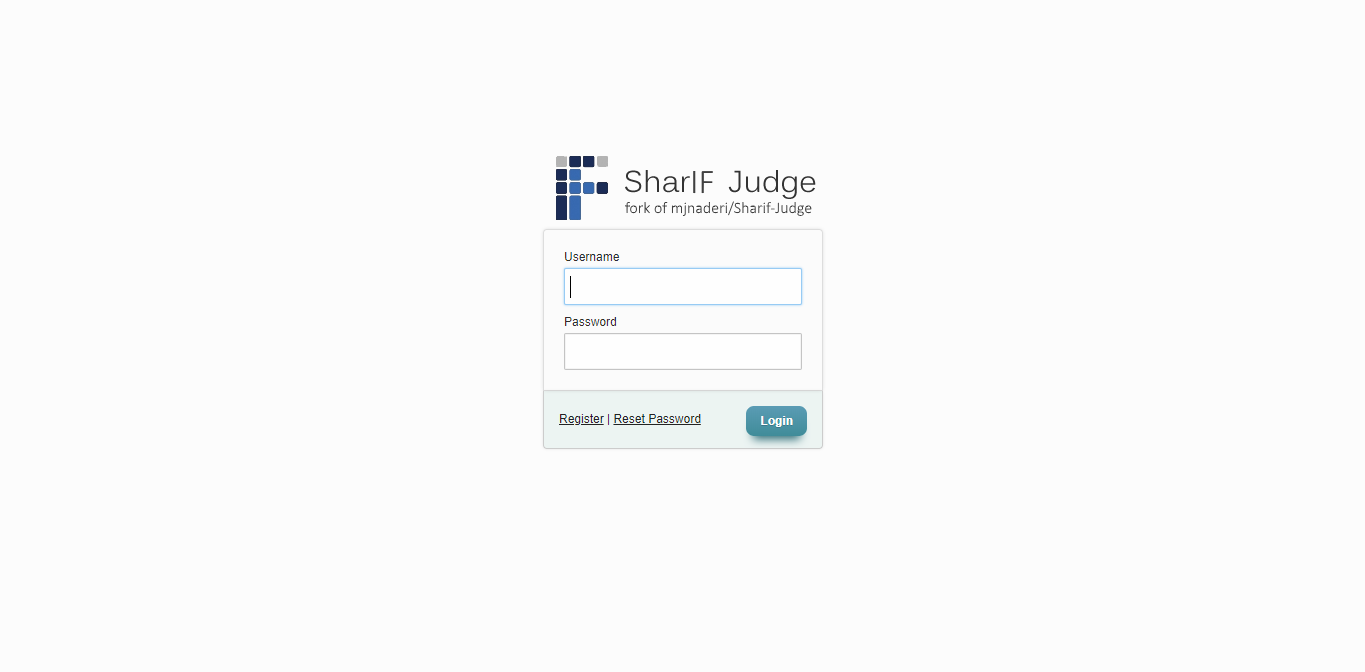
\includegraphics[width=1.0\textwidth]{newlogin}  
		\caption[Tampilan Halaman Login]{Tampilan Halaman \textit{Login}} 
		\label{fig:newlogin} 
	\end{figure}

	Gambar \ref{fig:newhof} menunjukan tampilan halaman \textit{Hall of Fame}.
	\begin{figure}[H]
		\centering  
		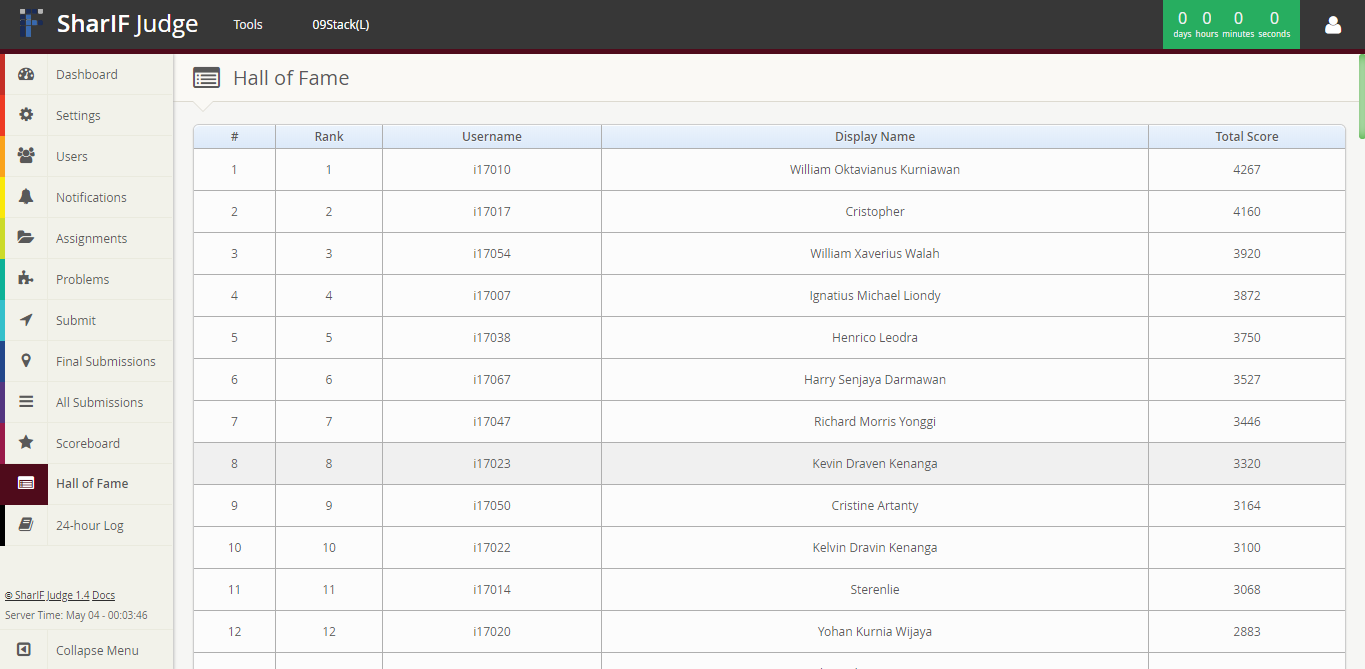
\includegraphics[width=1.0\textwidth]{/pengujian/hof/hof}  
		\caption[Tampilan Halaman Hall of Fame]{Tampilan Halaman \textit{Hall of Fame}} 
		\label{fig:newhof} 
	\end{figure}

	Gambar \ref{fig:newhofdetail} menunjukan tampilan \textit{detail} dari \textit{Hall of Fame}.
	\begin{figure}[H]
		\centering  
		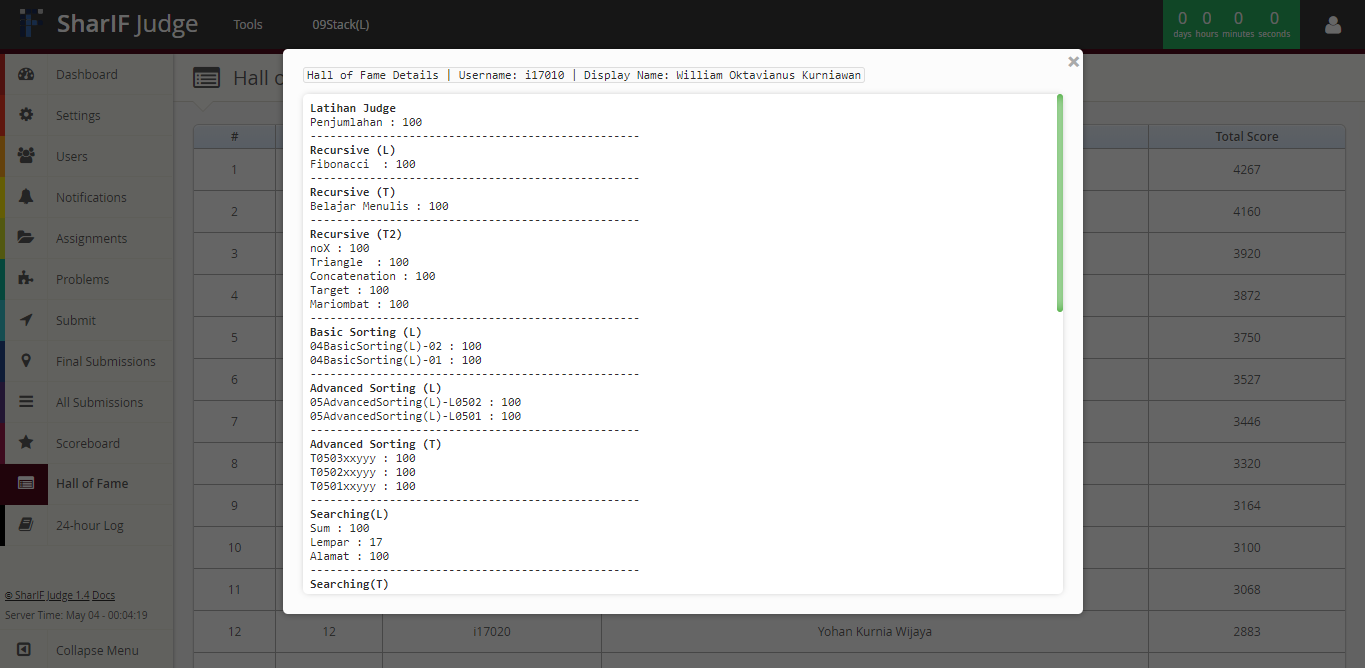
\includegraphics[width=1.0\textwidth]{/pengujian/hof/detailhof}  
		\caption[Tampilan Detail dari Hall of Fame]{Tampilan \textit{Detail} dari \textit{Hall of Fame}} 
		\label{fig:newhofdetail} 
	\end{figure}

	Gambar \ref{fig:newlogs} menunjukan tampilan halaman \textit{24-hour Logs}.
	\begin{figure}[H]
		\centering  
		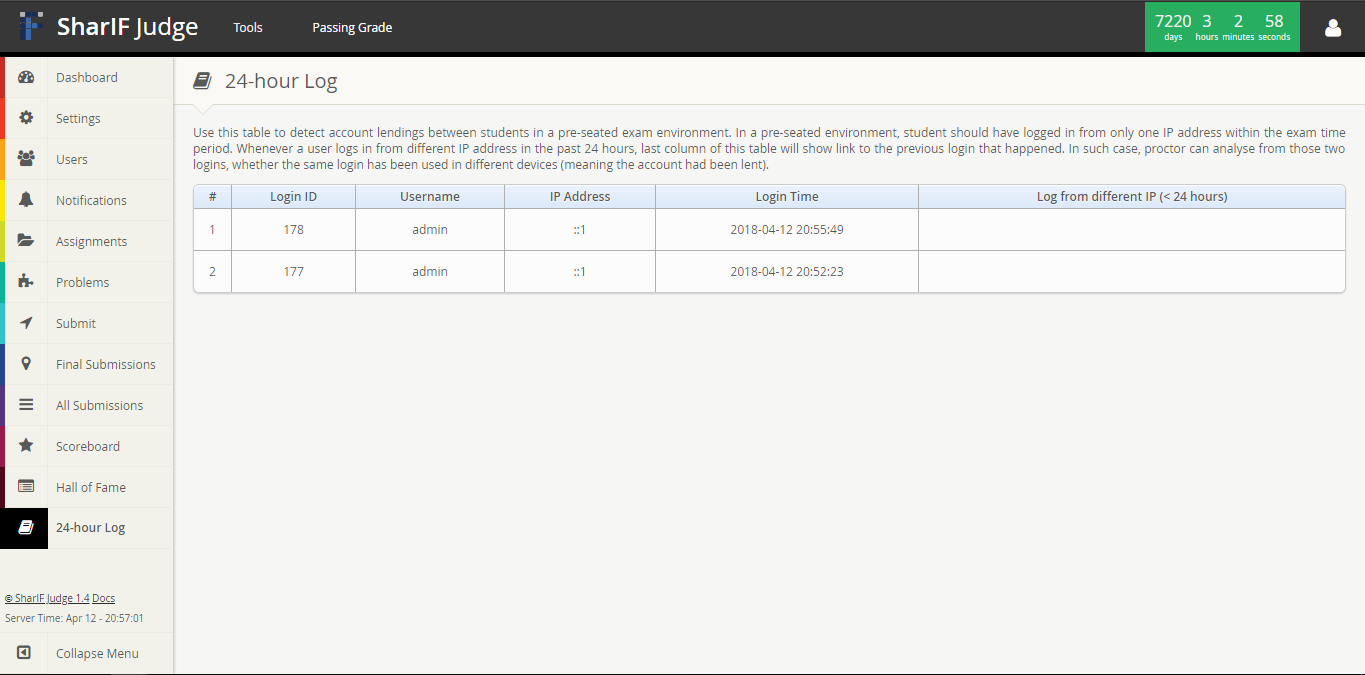
\includegraphics[width=1.0\textwidth]{newlogs}  
		\caption[Tampilan Halaman \textit{24-hour Logs}]{Tampilan Halaman \textit{24-hour Logs}} 
		\label{fig:newlogs} 
	\end{figure}
	
	Gambar \ref{fig:sidemenu} menunjukan tampilan \textit{side menu SharIF Judge}.
	\begin{figure}[H]
		\centering  
		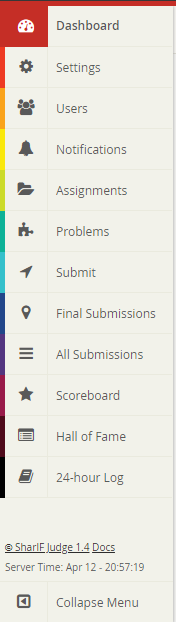
\includegraphics[scale=0.7]{sidemenu}  
		\caption[Tampilan\textit{ Side Menu SharIF Judge}]{Tampilan \textit{Side Menu SharIF Judge}} 
		\label{fig:sidemenu} 
	\end{figure}
	
	Gambar \ref{fig:ikons} menunjukan tampilan Ikon \textit{SharIF Judge} pada \textit{Title Bar}.
	\begin{figure}[H]
		\centering  
		
\includegraphics[scale=1]{ikon}  
		\caption[Ikon \textit{SharIF Judge} pada \textit{Title Bar}]{Ikon \textit{SharIF Judge} pada \textit{Title Bar}} 
		\label{fig:ikons} 
	\end{figure} 
	
	Gambar \ref{fig:logos} menunjukan tampilan Logo \textit{SharIF Judge} pada \textit{Top Bar}.
	\begin{figure}[H]
		\centering  
		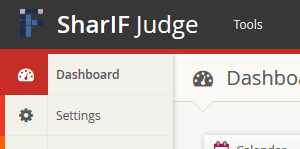
\includegraphics[scale=1]{logo}  
		\caption[Logo \textit{SharIF Judge} pada \textit{Top Bar}]{Logo \textit{SharIF Judge} pada \textit{Top Bar}} 
		\label{fig:logos} 
	\end{figure} 
\end{enumerate}

\section{Pengujian Fungsional}
%Pengujian fungsional bertujuan untuk memastikan bahwa perangkat lunak dapat berfungsi sebagaimana mestinya. Jika fungsi yang telah diimplementasi tidak berjalan dengan baik, maka perangkat lunak masih memiliki kekurangan.
Pengujian fungsional bertujuan untuk memastikan setiap fitur baru pada \textit{SharIF Judge} dapat berfungsi dengan baik.
	\subsection{Mengunduh Soal (deskripsi \& PDF) yang Telah Dibatasi} 
	Hasil yang diharapkan dari pengujian fitur ini adalah soal dapat dibatasi sesuai dengan ketentuan yang telah dirancang pada \hyperref[chap:batassoal]{sub bab 4.3}. Pengujian dimulai dengan membuat empat buah \textit{assignment}. Gambar \ref{fig:listassignment} menunjukan empat buah \textit{assignment} yang dibuat.
	\begin{figure}[H]
		\centering  
		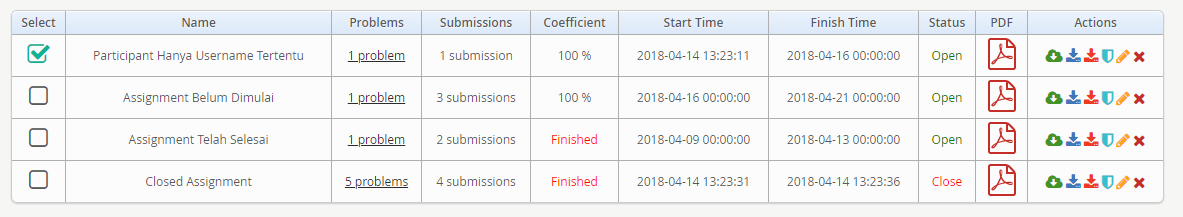
\includegraphics[width=1.0\textwidth]{/pengujian/batasisoal/listassignment}  
		\caption[Empat Buah \textit{Assignment} yang Dibuat]{Empat Buah \textit{Assignment} yang Dibuat} 
		\label{fig:listassignment} 
	\end{figure}
	
	\textit{Assignment} dengan nama "\textit{Participant} Hanya \textit{Username} Tertentu", merupakan \textit{assignment} yang dikhususkan untuk peserta tertentu. \textit{Assignment} dengan nama "\textit{Assignment} Belum Mulai", merupakan \textit{assignment} yang belum dimulai. \textit{Assignment} dengan nama "\textit{Assignment} Telah Selesai", merupakan \textit{assignment} yang waktu pengumpulannya telah habis. \textit{Assignment} dengan nama "\textit{Closed Assignment}", merupakan \textit{assignment} yang memiliki status \textit{close}. \\
	
	Jika peserta yang tidak terdaftar sebagai \textit{participant}, mencoba untuk mengunduh \textit{assignment} dengan nama "\textit{Participant} Hanya \textit{Username} Tertentu", maka muncul pesan \textit{error "You are not registered for submitting."} seperti \hyperref[fig:np]{Gambar 5.9} 
	\begin{figure}[H]
		\centering  
		
\includegraphics[width=1.0\textwidth]{/pengujian/batasisoal/np}  
		\caption[Pesan \textit{Error "You are not registered for submitting."}]{Pesan \textit{Error "You are not registered for submitting."}} 
		\label{fig:np} 
	\end{figure}

	Jika peserta mencoba untuk mengunduh \textit{assignment} dengan nama "\textit{Assignment} Belum Mulai", maka muncul pesan \textit{error "Selected assignment has not started."} seperti \hyperref[fig:ns]{Gambar 5.10} 
	\begin{figure}[H]
		\centering  
		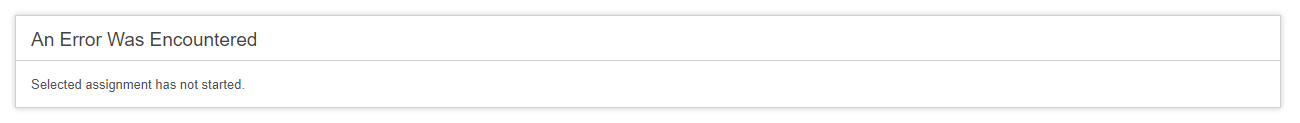
\includegraphics[width=1.0\textwidth]{/pengujian/batasisoal/ns}  
		\caption[Pesan \textit{Error "Selected assignment has not started."}]{Pesan \textit{Error "Selected assignment has not started."}} 
		\label{fig:ns} 
	\end{figure}

	Jika peserta mencoba untuk mengunduh \textit{assignment} dengan nama "\textit{Assignment} Telah Selesai", maka muncul pesan \textit{error "Selected assignment has finished."} seperti \hyperref[fig:f]{Gambar 5.11} 
	\begin{figure}[H]
		\centering  
		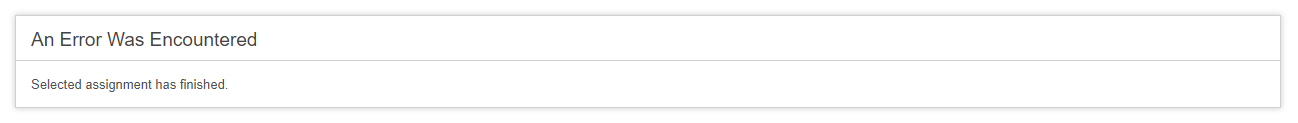
\includegraphics[width=1.0\textwidth]{/pengujian/batasisoal/f}  
		\caption[Pesan\textit{ Error "Selected assignment has finished."}]{Pesan \textit{Error "Selected assignment has finished."}} 
		\label{fig:f} 
	\end{figure}

	Jika peserta mencoba untuk mengunduh \textit{assignment} dengan nama "\textit{Closed Assignment}", maka muncul pesan \textit{error "Selected assignment has been closed."} seperti \hyperref[fig:c]{Gambar 5.12} 
	\begin{figure}[H]
		\centering  
		
\includegraphics[width=1.0\textwidth]{/pengujian/batasisoal/c}  
		\caption[Pesan \textit{Error "Selected assignment has been closed."}]{Pesan \textit{Error "Selected assignment has been closed."}} 
		\label{fig:c} 
	\end{figure}

	\subsection{Membuat \textit{Assignment} yang Menerima \textit{File} dengan Ekstensi TXT}
	Hasil yang diharapkan dari pengujian fitur ini adalah \textit{assignment} yang dibuat bisa menerima \textit{file} dengan ekstensi TXT dan pengguna bisa mengumpulkan file dengan ekstensi TXT ke \textit{assignment} tersebut. Pengujian dimulai dengan membuat \textit{assignment} yang bersifat "\textit{Upload Only}" dan menambahkan '\textit{txt}' pada \textit{text field Allowed Language}.
	\hyperref[fig:uploadtxt]{Gambar 5.13} menunjukan pembuatan \textit{assignment upload} TXT
	\begin{figure}[H]
		\centering  
		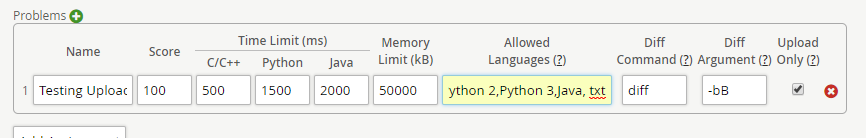
\includegraphics[width=1.0\textwidth]{/pengujian/uploadtxt/uploadtxt}  
		\caption[Pembuatan \textit{Assignment Upload} TXT]{Pembuatan \textit{Assignment Upload} TXT} 
		\label{fig:uploadtxt} 
	\end{figure}
	
	Setelah \textit{assignment} berhasil dibuat, selanjutnya dicoba untuk mengumpulkan \textit{file} dengan ekstensi TXT pada halaman \textit{Submit} seperti \hyperref[fig:submittxt]{Gambar 5.14}. Jika berhasil mengumpulkan \textit{file} TXT, maka pengguna langsung diarahkan ke halaman \textit{All Submission} seperti \hyperref[fig:resultttxt]{Gambar 5.15}
	
	\begin{figure}[H]
		\centering  
		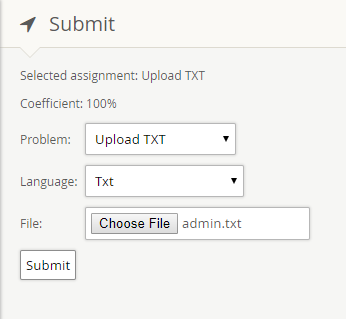
\includegraphics[scale=0.5]{/pengujian/uploadtxt/submittxt}  
		\caption[\textit{Submit File} TXT]{\textit{Submit File} TXT} 
		\label{fig:submittxt} 
	\end{figure}

	\begin{figure}[H]
		\centering  
		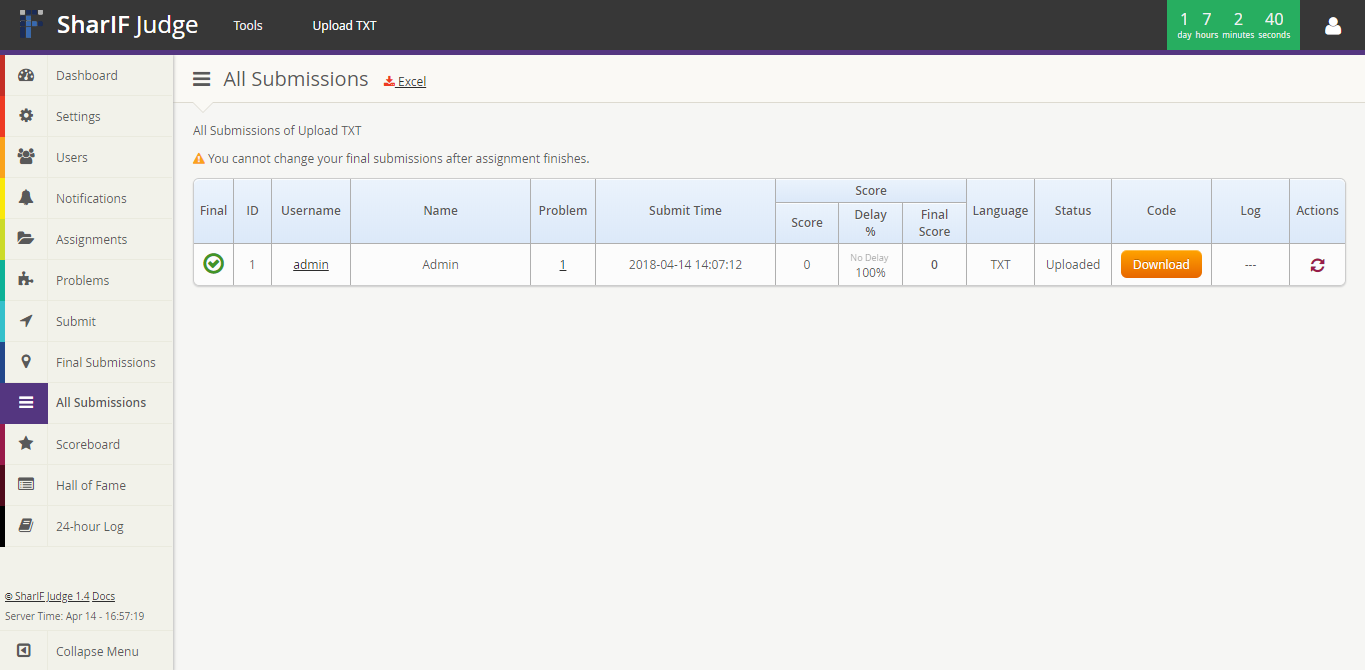
\includegraphics[width=1.0\textwidth]{/pengujian/uploadtxt/resulttxt}  
		\caption[Halaman \textit{All Submission} setelah Mengumpulkan \textit{File} TXT]{Halaman \textit{All Submission} setelah Mengumpulkan \textit{File} TXT} 
		\label{fig:resultttxt} 
	\end{figure}

	Pengujian dilanjutkan dengan mengunduh dan mencocokan isi dari \textit{file} TXT yang baru saja dikumpulkan. Jika isi dari \textit{file} TXT hasil unduh sama dengan \textit{file} TXT utama, maka fitur ini dapat berjalan dengan baik. \hyperref[fig:fileunduh]{Gambar 5.16} merupakan isi dari \textit{file} TXT hasil unduh dan \hyperref[fig:fileutama]{Gambar 5.17} isi dari \textit{file} TXT utama.
	
	\begin{figure}[H]
		\centering  
		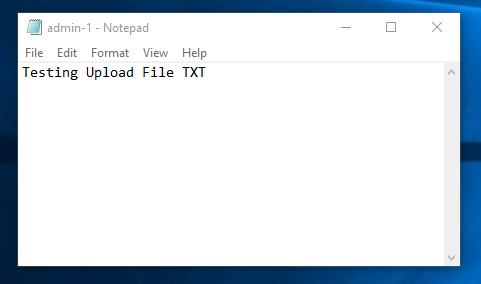
\includegraphics[scale=0.5]{/pengujian/uploadtxt/fileunduh}  
		\caption[\textit{File} TXT Hasil Unduh]{\textit{File} TXT Hasil Unduh} 
		\label{fig:fileunduh} 
	\end{figure}
	
	\begin{figure}[H]
		\centering  
		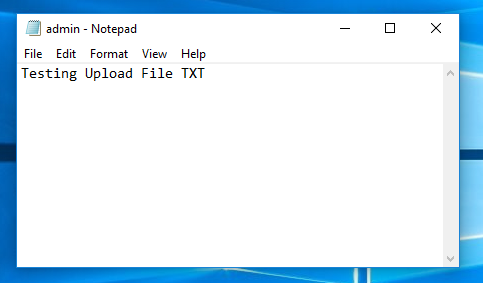
\includegraphics[scale=0.5]{/pengujian/uploadtxt/fileutama}  
		\caption[File TXT Utama]{File TXT Utama} 
		\label{fig:fileutama} 
	\end{figure}

	\subsection{Mengakses Halaman \textit{24-hour Logs}}
	Hasil yang diharapkan dari pengujian fitur ini adalah halaman \textit{24-hour Logs} dapat menampilkan seluruh aktivitas \textit{login} dari pengguna. Pengujian dimulai dari \textit{login} menggunakan \textit{username} dengan \textit{role admin}. Setelah berhasil \textit{login}, akses halaman \textit{24-hour Logs} yang terletak di paling bawah \textit{side menu}. Halaman \textit{24-hour Logs} tampil seperti \hyperref[fig:logs]{Gambar 5.18}
	\begin{figure}[H]
		\centering  
		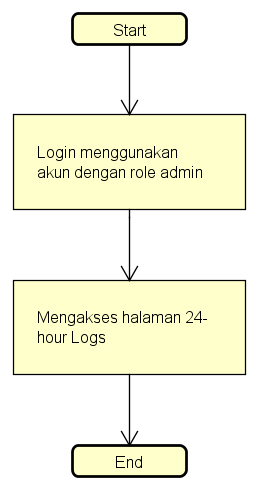
\includegraphics[width=1.0\textwidth]{/pengujian/logs/logs}  
		\caption[Halaman \textit{24-hour Logs} yang Tampil]{Halaman \textit{24-hour Logs} yang Tampil} 
		\label{fig:logs} 
	\end{figure}

	Pengujian dilanjutkan dengan mencoba \textit{login} menggunakan \textit{username} yang sama namun menggunakan \textit{ip address} yang berbeda. Hasil yang diharapkan adalah halaman \textit{24-hour Logs} dapat mencatat dan menampilkan \textit{Login ID} yang menggunakan \textit{ip address} berbeda.
	\begin{figure}[H]
		\centering  
		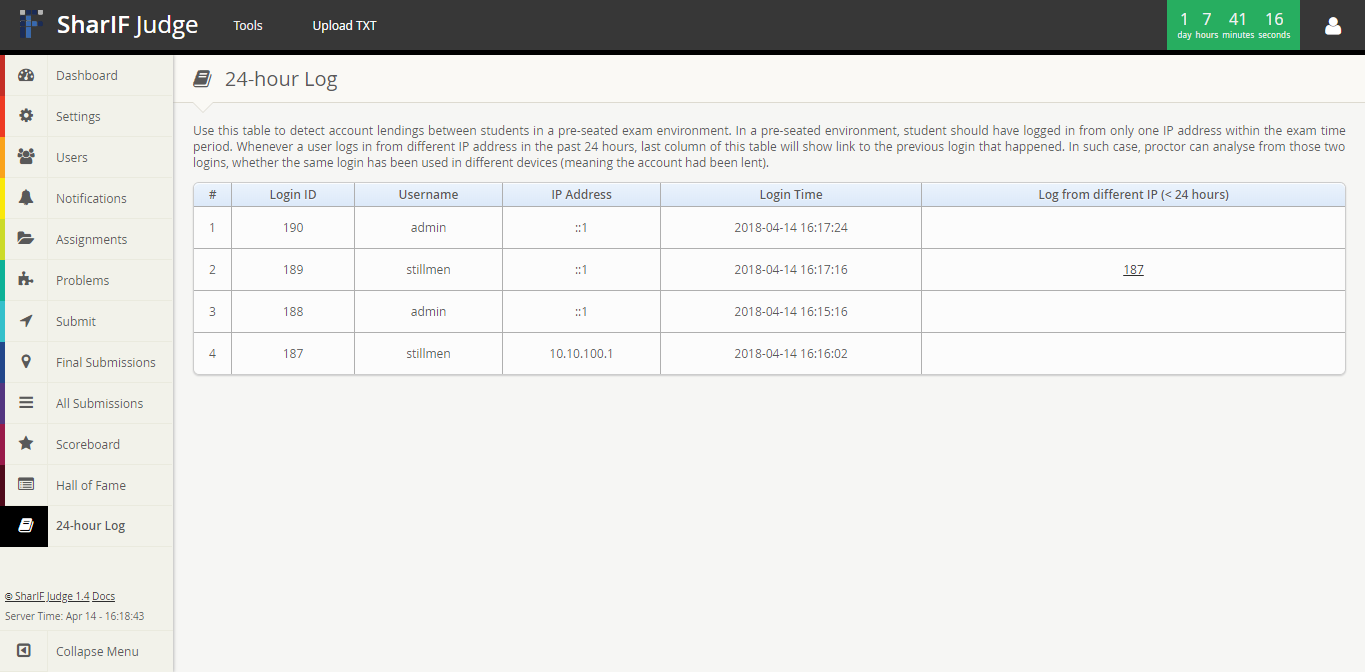
\includegraphics[width=1.0\textwidth]{/pengujian/logs/logs1}  
		\caption[Halaman \textit{24-hour Logs} Mencatat Aktivitas \textit{Login} Pengguna]{Halaman \textit{24-hour Logs} Mencatat Aktivitas \textit{Login} Pengguna} 
		\label{fig:logs1} 
	\end{figure}
	Terlihat pada \hyperref[fig:logs1]{Gambar 5.19}, \textit{username} stillmen pertama kali \textit{login} menggunakan \textit{ip address} 172.68.253.50 (baris 2). Setelah mencoba untuk \textit{login} menggunakan \textit{ip address} yang berbeda, halaman \textit{24-hour Logs} dapat mencatat dan menampilkan \textit{Login ID} dari \textit{username} stillmen (baris 1).
	
	\subsection{Mendaftarkan Peserta Menggunakan Tambahan Parameter "\textit{Display Name}"}
	Hasil yang diharapkan dari pengujian fitur ini adalah peserta yang didaftarkan langsung memiliki \textit{Display Name}. Pengujian dimulai dengan menekan tombol \textit{Add Users} pada halaman \textit{Users}. Gunakan parameter "pengguna1,pengguna1@judge.com,Pengguna Satu,penggunaa1,student" untuk menambah peserta baru seperti \hyperref[fig:useradd]{Gambar 5.20}
	\begin{figure}[H]
		\centering  
		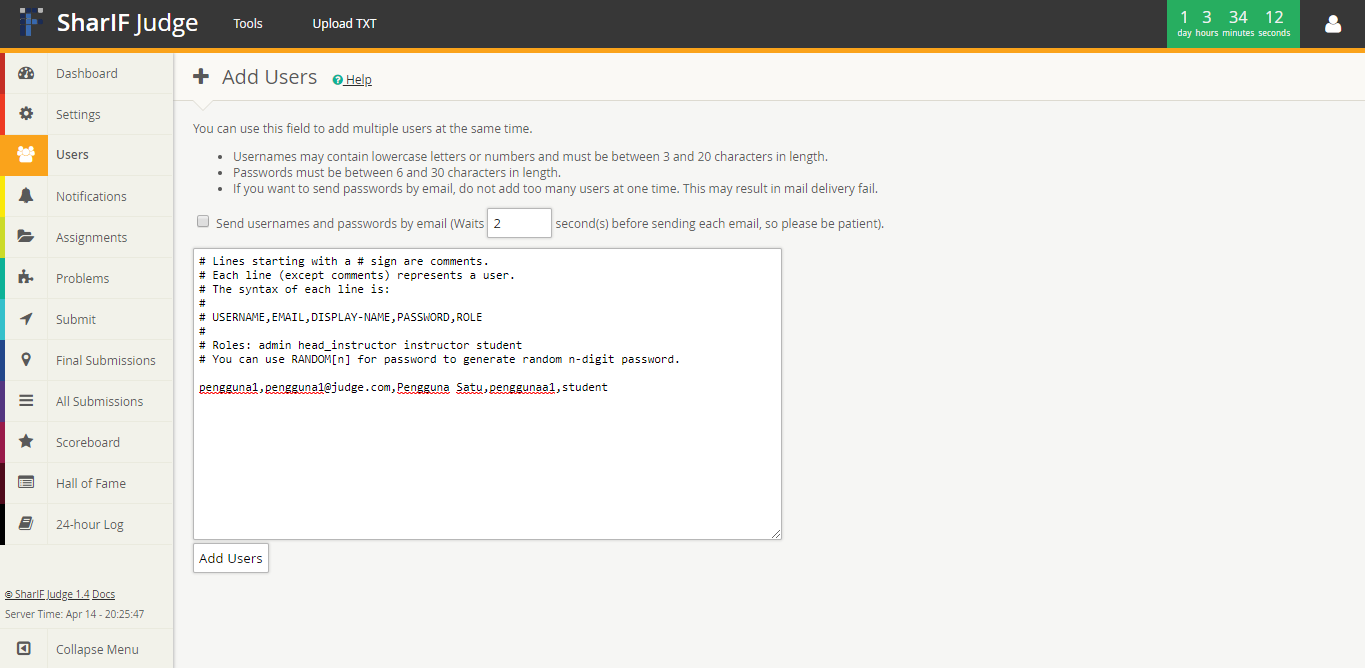
\includegraphics[width=1.0\textwidth]{/pengujian/displayname/add}  
		\caption[Halaman \textit{Add User}]{Halaman \textit{Add User}} 
		\label{fig:useradd} 
	\end{figure}

	Jika pengguna baru berhasil ditambahkan, maka akan muncul pesan bahwa tersebut berhasil didaftarkan seperti \hyperref[fig:success]{Gambar 5.21}
	\begin{figure}[H]
		\centering  
		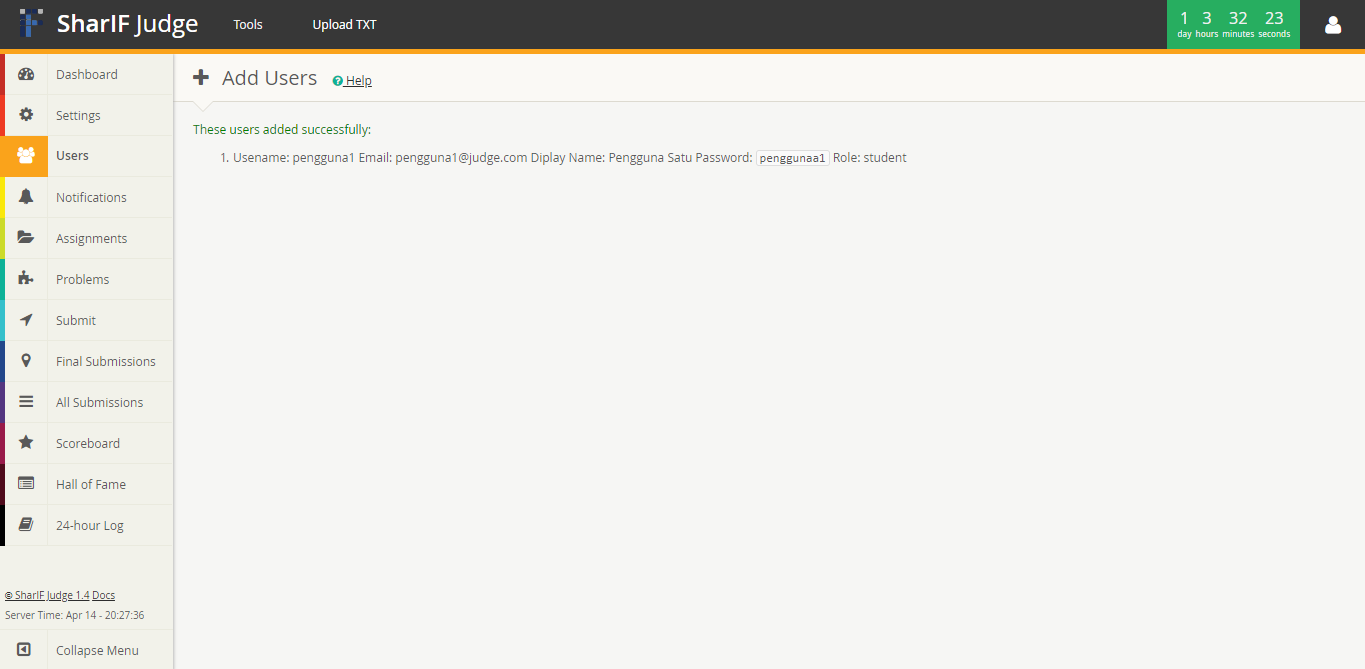
\includegraphics[width=1.0\textwidth]{/pengujian/displayname/success}  
		\caption[Pengguna Berhasil Didaftarkan]{Pengguna Berhasil Didaftarkan} 
		\label{fig:success} 
	\end{figure}

	Pengujian dilanjutkan dengan \textit{login} menggunakan \textit{user} yang baru didaftarkan dan mengecek \textit{Display Name}. \hyperref[fig:dp]{Gambar 5.22} menunjukan bahwa \textit{Display Name} yang muncul sesuai dengan parameter \textit{Display Name} yang telah dimasukan sebelumnya.
	\begin{figure}[H]
		\centering  
		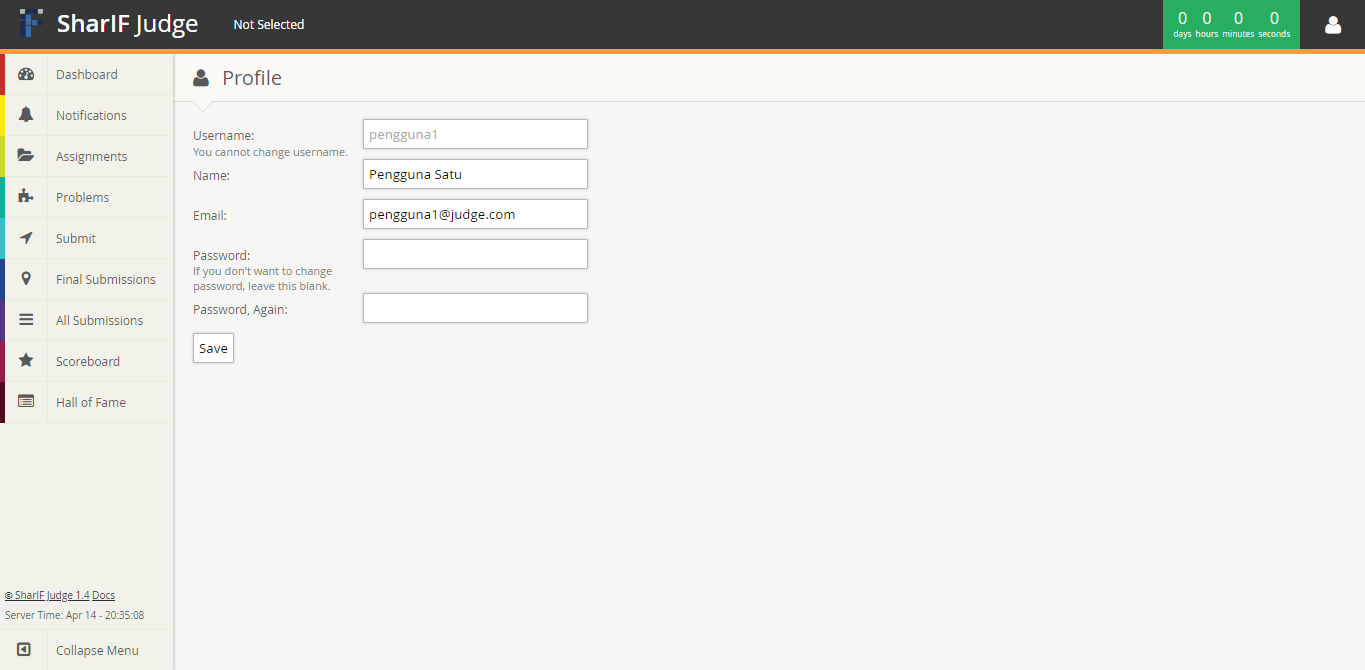
\includegraphics[width=1.0\textwidth]{/pengujian/displayname/dp}  
		\caption[\textit{Display Name} yang Tampil Sesuai dengan Parameter yang Dimasukan]{\textit{Display Name} yang Tampil Sesuai dengan Parameter yang Dimasukan} 
		\label{fig:dp} 
	\end{figure}

	\subsection{\textit{Disable Display Name} Peserta Menggunakan Fitur "\textit{Lock Student's Display Name}"}
	Hasil yang diharapkan dari pengujian fitur ini adalah \textit{text field Display Name} pada halaman \textit{Profile} menjadi \textit{disable}, sehingga para peserta tidak dapat mengubahnya. Pengujian dimulai dengan mengaktifkan fitur \textit{Lock Student's Display Name} pada halaman \textit{Settings} seperti \hyperref[fig:aktif]{Gambar 5.23}.
	\begin{figure}[H]
		\centering  
		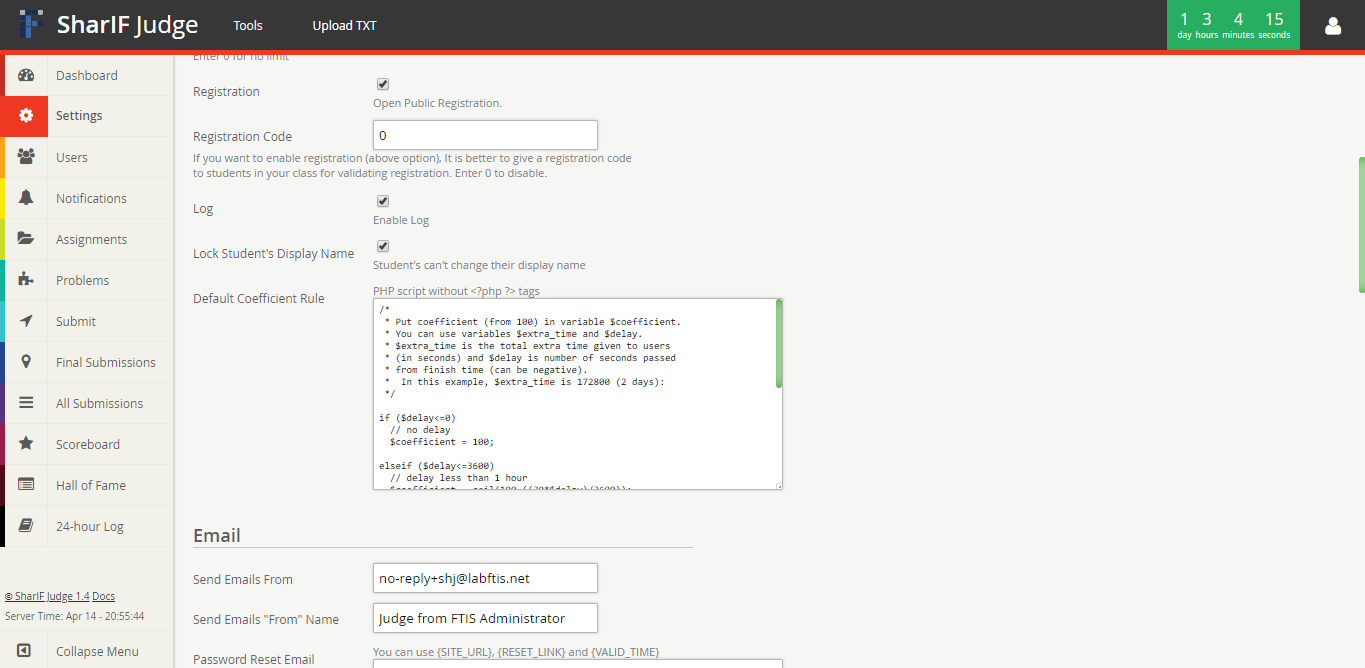
\includegraphics[width=1.0\textwidth]{/pengujian/lock/aktif}  
		\caption[Mengaktifkan Fitur \textit{Lock Student's Display Name}]{Mengaktifkan Fitur \textit{Lock Student's Display Name}} 
		\label{fig:aktif} 
	\end{figure}
	
	Pengujian dilanjutkan dengan mengecek \textit{text field Display Name} pada halaman \textit{Profile}. \hyperref[fig:disable]{Gambar 5.24} menunjukan bahwa \textit{text field Display Name} telah disable.
	\begin{figure}[H]
		\centering  
		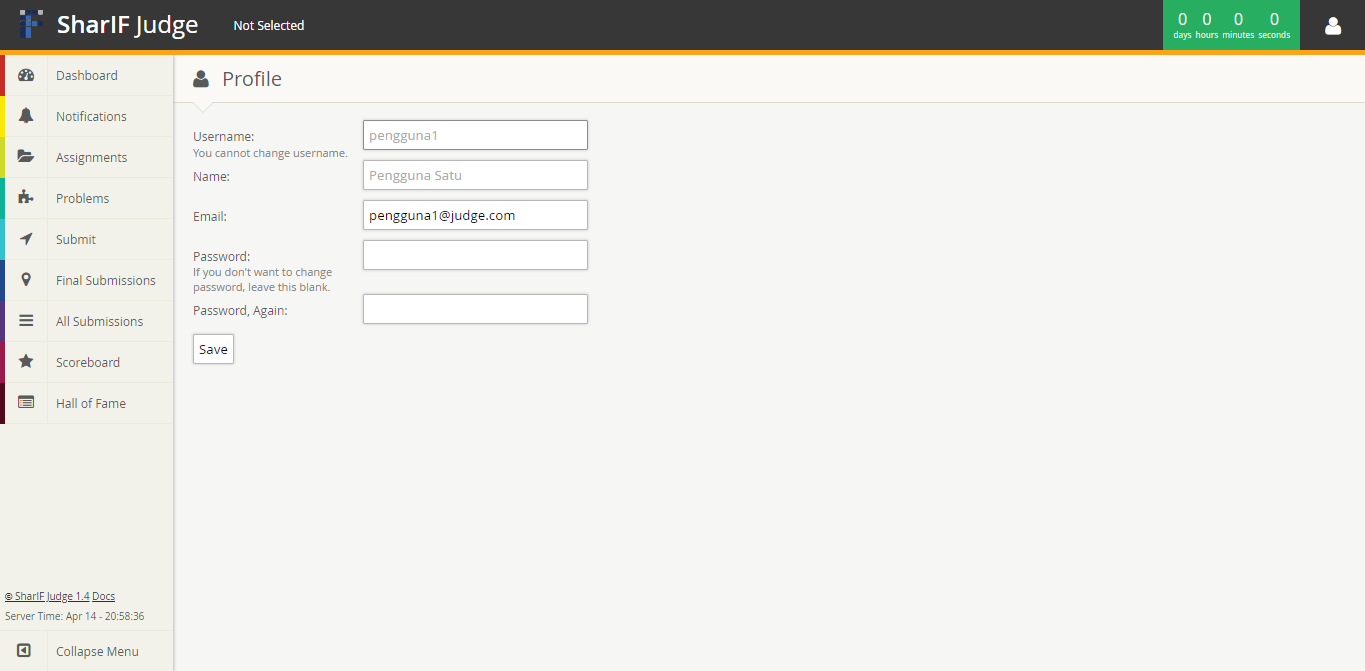
\includegraphics[width=1.0\textwidth]{/pengujian/lock/disable}  
		\caption[\textit{Text Field Display Name} Menjadi \textit{Disable}]{\textit{Text Field Display Name} Menjadi \textit{Disable}} 
		\label{fig:disable} 
	\end{figure}

	\subsection{Menambahkan \textit{Assignment} yang Mengaktifkan Fitur "\textit{Archived Assignment}"}
	Hasil yang diharapkan dari pengujian fitur ini adalah \textit{\textit{assignment}} yang diibuat memiliki batas waktu pengumpulan sampai tanggal 18 Januari 2038. Pengujian dimulai dengan membuat \textit{assignment} dan mengaktifkan fitur \textit{Archived Assignment} pada halaman \textit{Add Assignment} seperti \hyperref[fig:arc]{Gambar 5.25}.
	\begin{figure}[H]
		\centering  
		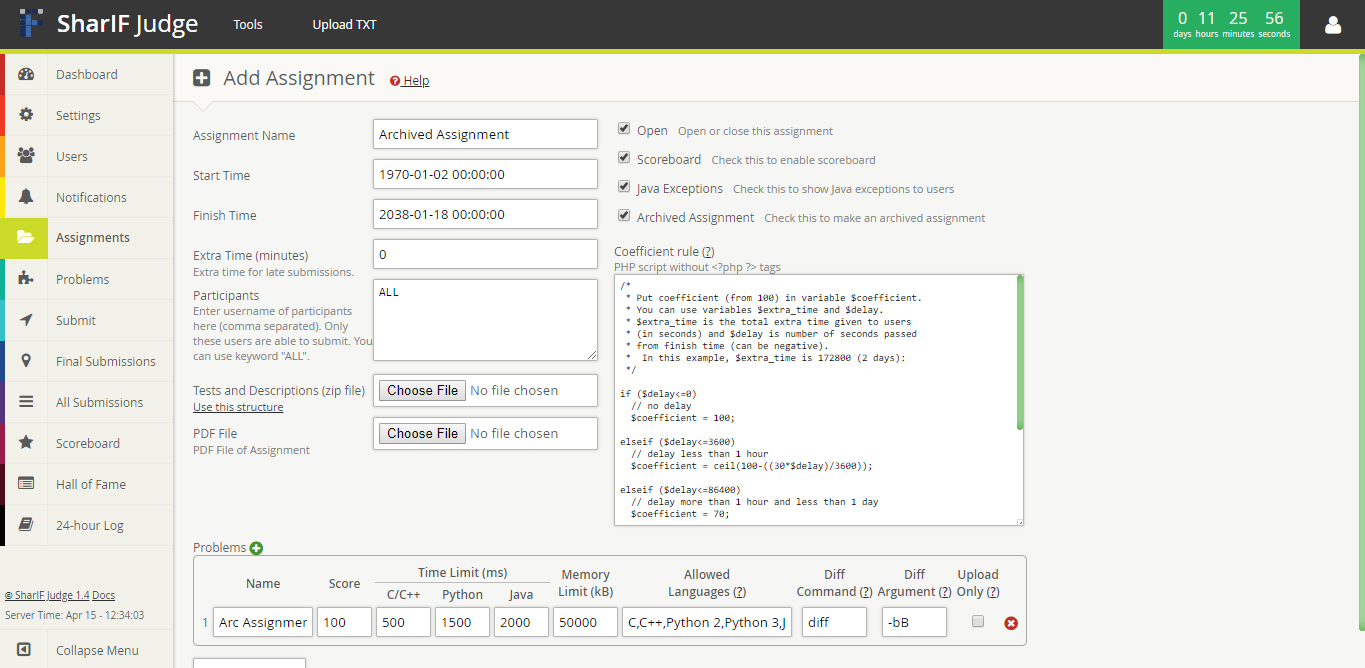
\includegraphics[width=1.0\textwidth]{/pengujian/arcass/addarc}  
		\caption[Mengaktifkan Fitur \textit{Archived Assignment}]{Mengaktifkan Fitur \textit{Archived Assignment}} 
		\label{fig:arc} 
	\end{figure}
	
	\hyperref[fig:listarc]{Gambar 5.26} menunjukan bahwa \textit{assignment} yang baru dibuat (baris 1) memiliki nilai \textit{Finish Time} "2038-01-18 00:00:00" yang artinya \textit{assignment} tersebut dapat dikumpulkan sampai tanggal 18 Januari 2038.
	\begin{figure}[H]
		\centering  
		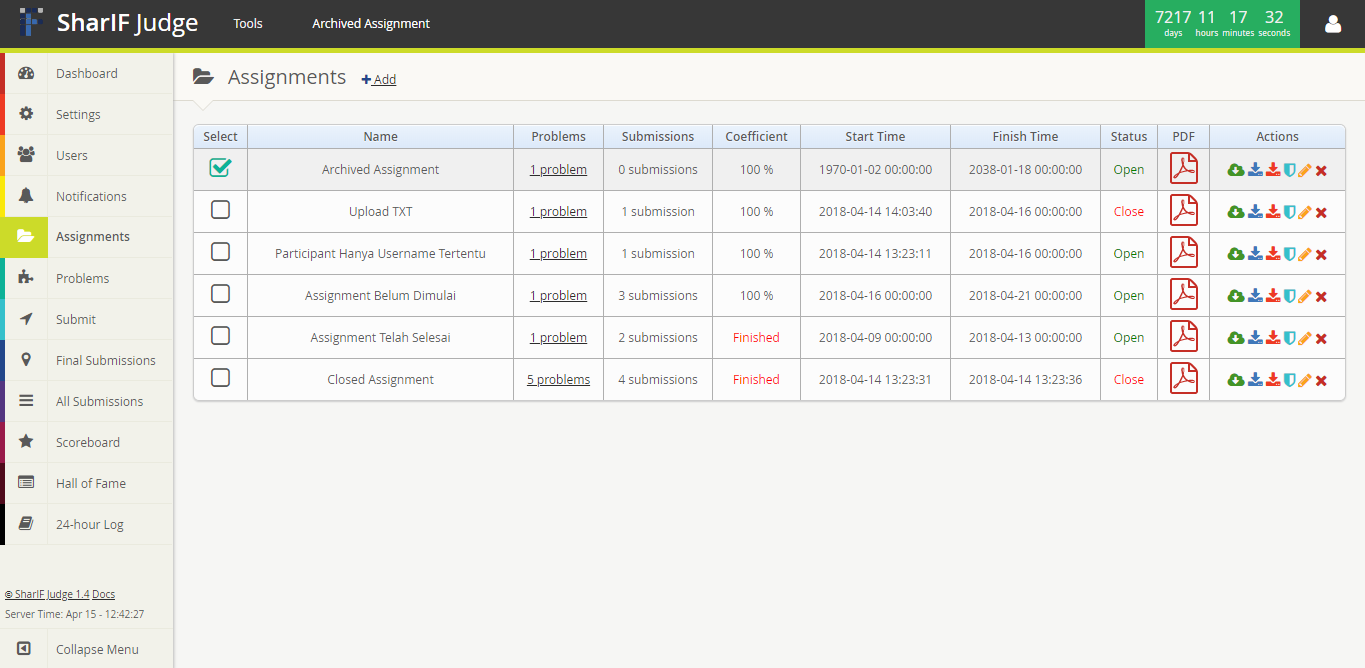
\includegraphics[width=1.0\textwidth]{/pengujian/arcass/listarc}  
		\caption[\textit{Finish Time} dengan Nilai "2038-01-18 00:00:00"]{\textit{Finish Time} dengan Nilai "2038-01-18 00:00:00"} 
		\label{fig:listarc} 
	\end{figure}

	Pengujian dilanjutkan dengan mengecek kalendar pada halaaman \textit{Dashboard}. \textit{Assignment} yang mengaktifkan fitur \textit{Archived Assignment} tidak akan muncul pada kalendar seperti \hyperref[fig:kalarc]{Gambar 5.27}
	\begin{figure}[H]
		\centering  
		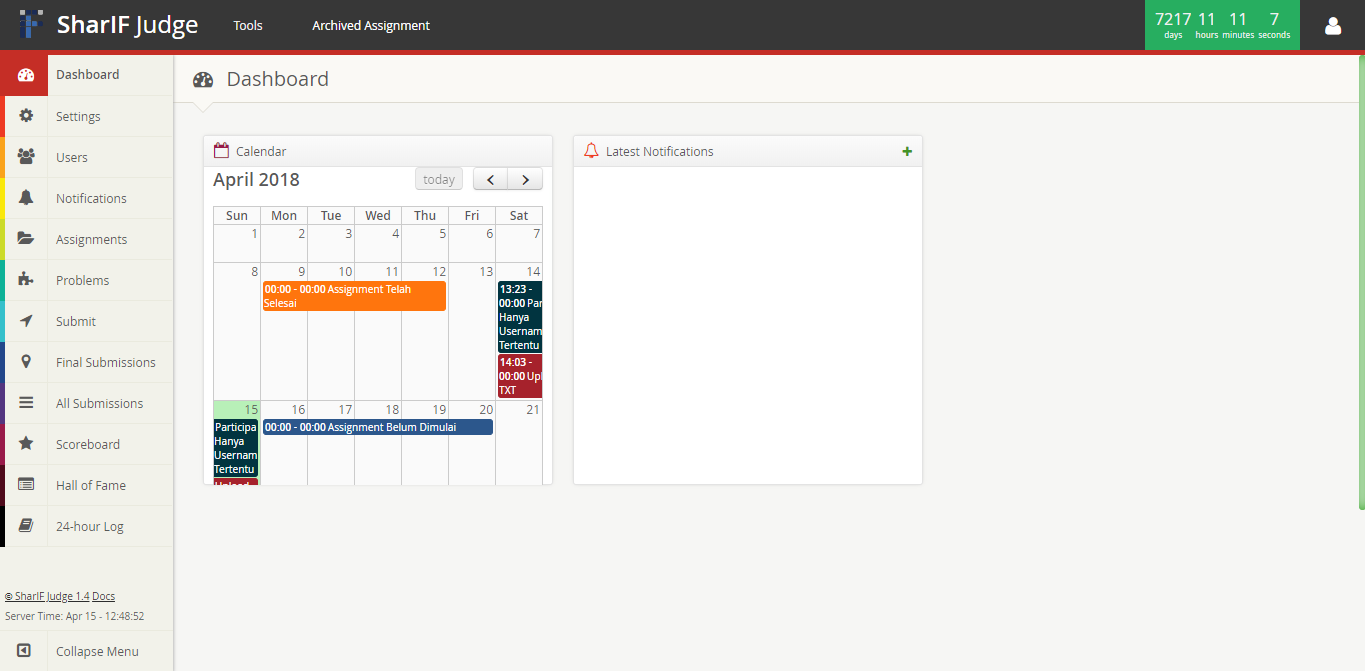
\includegraphics[width=1.0\textwidth]{/pengujian/arcass/kalarc}  
		\caption[\textit{Archived Assignment} Tidak Muncul pada Kalendar]{\textit{Archived Assignment} Tidak Muncul pada Kalendar} 
		\label{fig:kalarc} 
	\end{figure}

	\subsection{Mengakses Halaman \textit{Hall of Fame}}
	Hasil yang diharapkan dari pengujian fitur ini adalah halaman \textit{Hall of Fame} dapat menampilkan total nilai semua pengguna dari setiap \textit{assignment} yang telah dikumpulkan. Pengujian dimulai dengan mengakses halaman \textit{Hall of Fame} yang terletak di bawah \textit{side menu Scoreboard}. Halaman \textit{Hall of Fame} tampil seperti \hyperref[fig:halhof]{Gambar 5.28}
	\begin{figure}[H]
		\centering  
		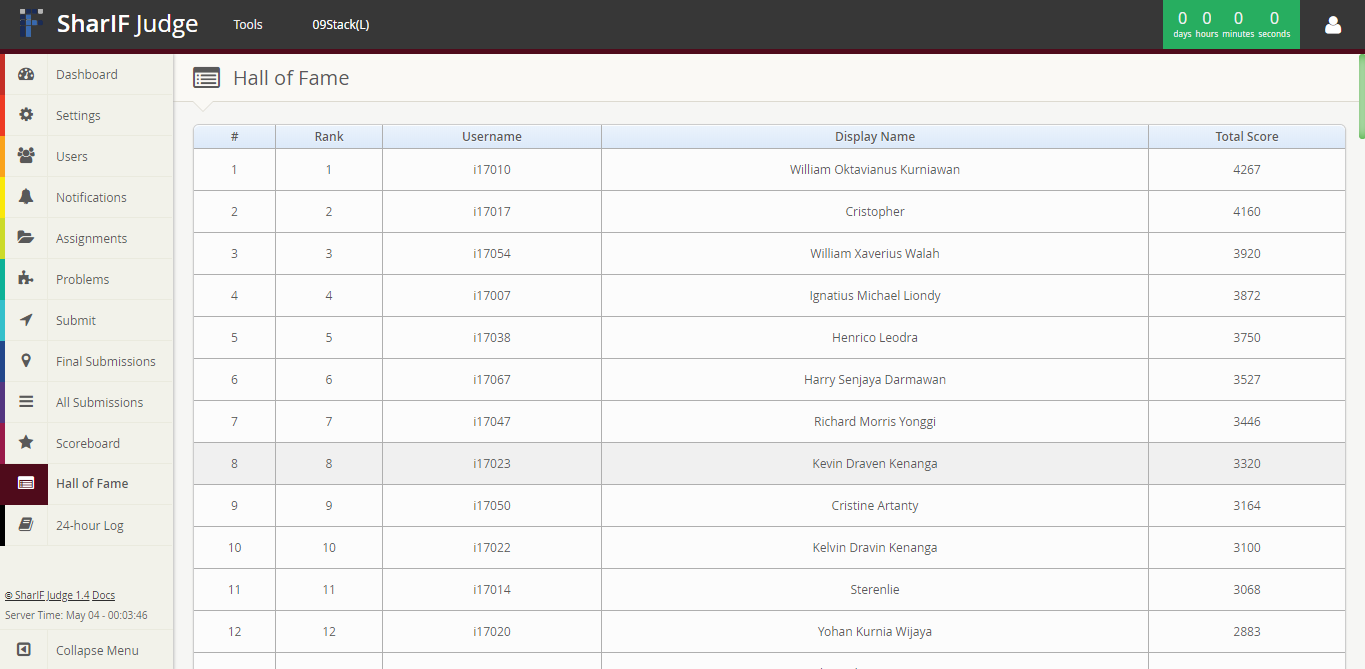
\includegraphics[width=1.0\textwidth]{/pengujian/hof/hof}  
		\caption[Halaman \textit{Hall of Fame}]{Halaman \textit{Hall of Fame}} 
		\label{fig:halhof} 
	\end{figure}

	Pengujian dilanjutkan dengan mengklik baris pada tabel untuk melihat \textit{details} nilai pengguna. \hyperref[fig:dethof]{Gambar 5.29} menunjukan \textit{details} nilai yang diperoleh pengguna dengan \textit{username i17010}.
	\begin{figure}[H]
		\centering  
		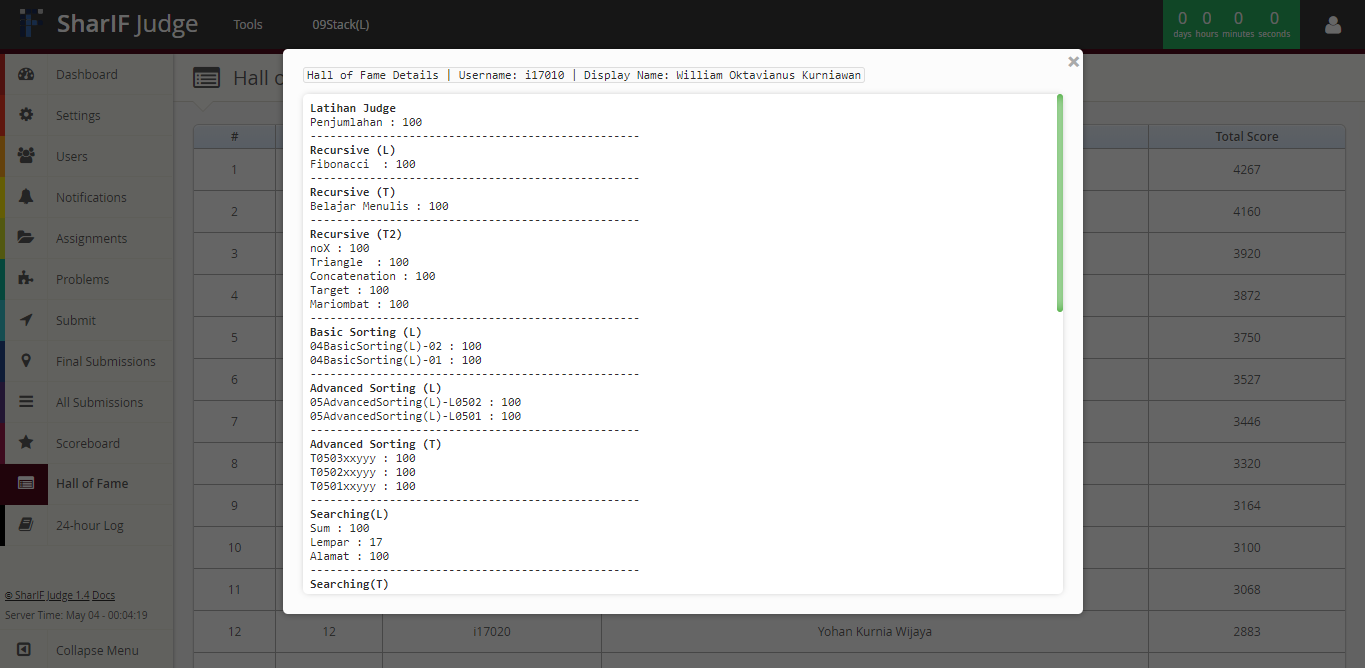
\includegraphics[width=1.0\textwidth]{/pengujian/hof/detailhof}  
		\caption[\textit{Details} Nilai yang Diperoleh]{\textit{Details} Nilai yang Diperoleh} 
		\label{fig:dethof} 
	\end{figure}
	
\section{Pengujian Ekseprimental}
Pengujian eksperimental dilakukan dengan cara menginstal perangkat lunak \textit{SharIF Judge} pada server lab FTIS UNPAR. Pengujian ini bertujuan untuk menguji secara langsung fitur-fitur baru \textit{SharIF Judge} pada mata kuliah pemrograman. \textit{SharIF Judge} diuji untuk mata kuliah Algoritma \& Struktur Data (ASD) semester genap 2017/2018. \textit{SharIF Judge} yang telah diinstall, dapat diakses pada \textit{URL} \path{http://asd-lat.ftis.unpar/} dan \path{http://asd-quiz.ftis.unpar/}. Selama pengujian berlangsung, terdapat beberapa persoalan yang muncul. Persoalan yang muncul dicatat ke dalam \textit{issue} \textit{repository SharIF Judge} di \textit{GitHub}. Semua persoalan dapat dilihat di \path{https://github.com/ayenz/Sharif-Judge/issues}.

	\subsection{\textit{Remove the Assignments Folder}}
	\textit{Issue} dengan kode unik \#4 meminta agar \textit{folder assignments} untuk dihapus. Hal ini bertujuan agar direktori \textit{URL} \path{/assignments} dapat diakses. \textit{Folder assignments} merupakan \textit{folder default} untuk menyimpan \textit{assignment}. \textit{Folder default} penyimpanan \textit{assignment} tersebut harus diubah terlebih dahulu. Untuk mengubah \textit{folder default} penyimpanan, diperlukan perubahan nilai pada halaman \textit{Settings} dan kode pada kelas \textit{Controller Install.php}. Selain mengubah \textit{folder default} penyimpanan \textit{assignment}, perubahan juga dilakukan pada \textit{folder default tester} dan \textit{default timezone} yang bertujuan untuk merapihkan struktur direktori.
	\begin{figure}[H]
		\centering  
		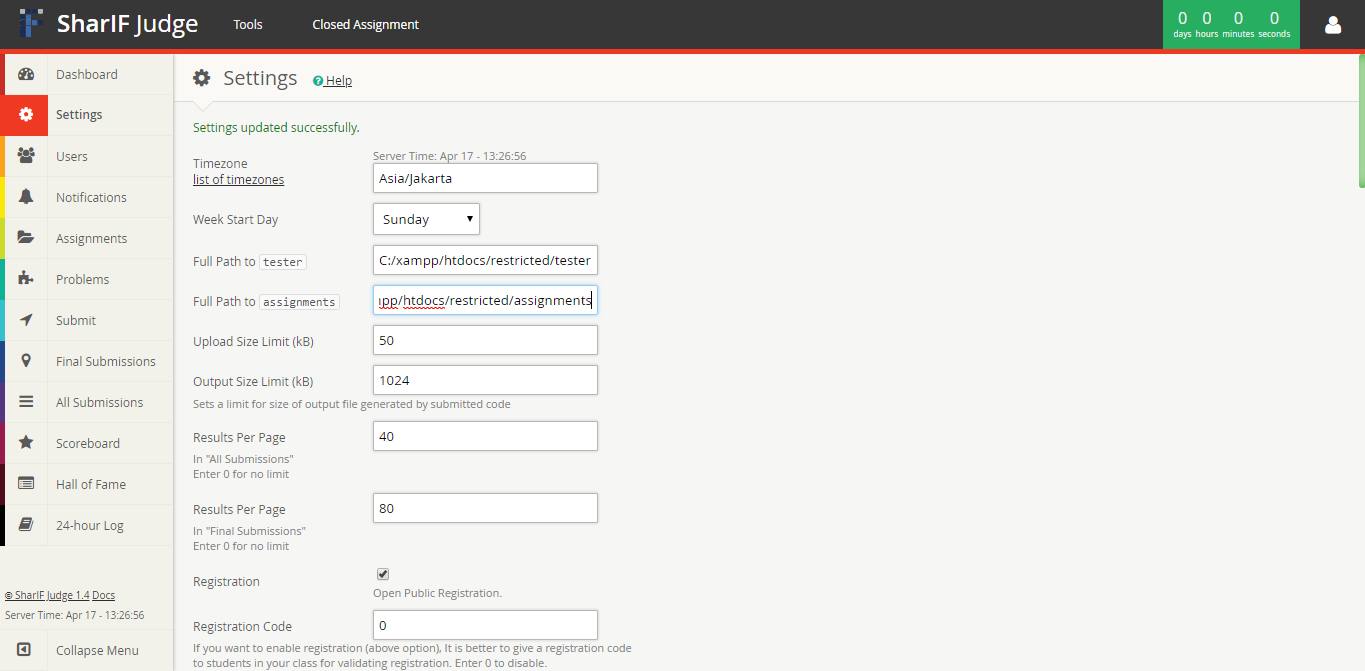
\includegraphics[width=1.0\textwidth]{/pengujian/set}  
		\caption[Perubahan yang Dilakukan pada Halaman \textit{Settings}]{Perubahan yang Dilakukan pada Halaman \textit{Settings}} 
		\label{fig:set} 
	\end{figure}
	
	\hyperref[fig:set]{Gambar 5.30} menunjukan perubahan pada halaman \textit{Settings} dilakukan pada \textit{text field} "\textit{Timezone}", "\textit{Full Path to tester}" dan "\textit{Full Path to assignments}". 
	\begin{itemize}
		\item Nilai yang digunakan untuk\textit{ text field "Full Path to assignments"} adalah \path{C:/xampp/htdocs/restricted/assignments}. Nilai tersebut memiliki arti bahwa \textit{folder default} penyimpanan \textit{assignment} diletakan pada direktori \path{C:/xampp/htdocs/restricted/assignments}.
		\item Nilai yang digunakan untuk \textit{text field "Full Path to tester"} adalah \path{C:/xampp/htdocs/restricted/tester}. Nilai tersebut memiliki arti bahwa \textit{folder default tester} diletakan pada direktori \path{C:/xampp/htdocs/restricted/tester}.
		\item Nilai yang digunakan untuk \textit{text field "Timezone"} adalah Asia/Jakarta. Nilai tersebut memiliki arti bahwa \textit{default timezone} yang digunakan pada \textit{SharIF Judge} mengikuti \textit{timezone} wilayah Asia/Jakarta.
	\end{itemize}
	
	Perubahan kode pada kelas \textit{Controller Install.php} bertujuan agar penginstalan \textit{SharIF Judge} langsung menggunakan \textit{default} nilai seperti di atas. Listing \ref{lstt:1} menunjukan perubahan kode program yang dilakukan di \textit{Install.php}
	
\begin{lstlisting}[language=diff, caption=Perubahan kode program pada \textit{Install.php}, label=lstt:1,basicstyle=\ttfamily, frame=single,
columns=fullflexible, keepspaces=true, breaklines=true]
@@ -196,9 +196,9 @@ class Install extends CI_Controller

// insert default settings to table 'settings'
$result = $this->db->insert_batch('settings', array(
-   	array('shj_key' => 'timezone',               'shj_value' => 'Asia/Tehran'),
-       array('shj_key' => 'tester_path',            'shj_value' => '/home/shj/tester'),
-       array('shj_key' => 'assignments_root',       'shj_value' => '/home/shj/assignments'),
+       array('shj_key' => 'timezone',               'shj_value' => 'Asia/Jakarta'),
+       array('shj_key' => 'tester_path',            'shj_value' => dirname(__FILE__, 3) . "/restricted/tester"),
+       array('shj_key' => 'assignments_root',       'shj_value' => dirname(__FILE__, 3) . "/restricted/assignments"),
\end{lstlisting}
	Setelah melakukan beberapa perubahan, folder assignment dapat dihapus.
	
	\subsection{\textit{Add User Email are not formatted correctly}}
	\textit{Issue} dengan kode unik \#5 mengatakan bahwa pendaftaran peserta via \textit{email} tidak berfungsi dengan baik. Pengguna mendapatkan \textit{email} dengan format yang tidak beraturan. Contohnya \textit{username} yang tertukar dengan \textit{role} dan \textit{password} tertukar dengan \textit{display name} seperti \hyperref[fig:dnve]{Gambar 5.31} 
	\begin{figure}[H]
		\centering  
		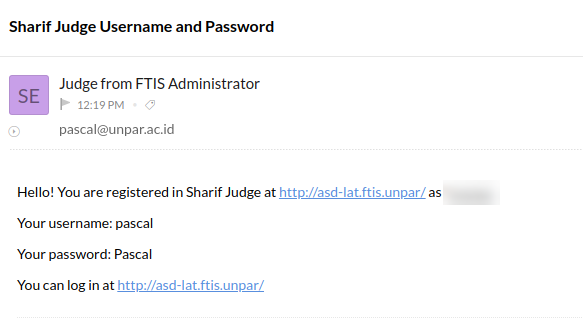
\includegraphics[width=1.0\textwidth]{/pengujian/dnve}  
		\caption[Format \textit{Email} Tidak Beraturan]{Format \textit{Email} Tidak Beraturan} 
		\label{fig:dnve} 
	\end{figure}

	Hal di atas terjadi karena penambahan parameter "\textit{Display Name}" pada fungsi \textit{add\_user} yang terdapat di \textit{model User\_model.php}. Persoalan ini dapat diatasi dengan memperbaiki urutan data yang dikirimkan ke email. Listing \ref{lstt:2} menunjukan perubahan kode program yang dilakukan di \textit{User\_model.php}
	
\begin{lstlisting}[language=diff, caption=Perubahan kode program pada \textit{User\_model.php}, label=lstt:2, basicstyle=\ttfamily, frame=single,
columns=fullflexible, keepspaces=true, breaklines=true]
@@ -219,9 +219,9 @@ class User_model extends CI_Model
	$this->email->subject('Sharif Judge Username and Password');
	$text = $this->settings_model->get_setting('add_user_mail');
	$text = str_replace('{SITE_URL}', base_url(), $text);
-   	$text = str_replace('{ROLE}', $user[3], $text);
+   	$text = str_replace('{ROLE}', $user[4], $text);
	$text = str_replace('{USERNAME}', $user[0], $text);
-   	$text = str_replace('{PASSWORD}', htmlspecialchars($user[2]), $text);
+   	$text = str_replace('{PASSWORD}', htmlspecialchars($user[3]), $text);
	$text = str_replace('{LOGIN_URL}', base_url(), $text);
	$this->email->message($text);
	$this->email->send();
\end{lstlisting}
	Setelah melakukan perubahan kode program, pendaftaran peserta via \textit{email} dapat berfungsi dengan baik. \textit{Email} yang diterima pengguna telah menggunakan format yang benar.
	
	\subsection{\textit{Cannot Create Assignments}}
	\textit{Issue} dengan kode unik \#7 mengatakan bahwa Bapak Husnul selaku dosen Algoritma \& Struktur Data, tidak bisa membuat \textit{assignment}.\textit{ Error log} yang dihasilkan tidak menunjukan pesan kesalahan apapun. 
	Berikut isi \textit{error log} yang terdapat di direktori \path{/var/log/apache2/error.log}
\begin{lstlisting}[basicstyle=\ttfamily, frame=single,columns=fullflexible, keepspaces=true, breaklines=true]
[Wed Jan 31 06:25:02.516154 2018] [mpm_prefork:notice] [pid 1734] AH00163: Apache/2.4.18 (Ubuntu) configured -- resuming normal operations
[Wed Jan 31 06:25:02.516182 2018] [core:notice] [pid 1734] AH00094: Command line: '/usr/sbin/apache2
\end{lstlisting}
	
	Persoalan terjadi karena tidak ada atribut \textit{archived\_assignment} di tabel \textit{shj\_assignments}. Persoalan ini dapat diatasi dengan menambahkan atribut \textit{archived\_assignment} di tabel \textit{shj\_assignments}, sehingga struktur tabel \textit{shj\_assignments} menjadi seperti \hyperref[tab:atributtabelassignments]{Tabel 5.5}. \textit{Assignment} berhasil dibuat setelah atribut \textit{archived\_assignment} ditambahkan.
	
	\subsection{\textit{Link} ke \textit{New Home of Sharif-Judge}}
	\textit{Issue} dengan kode unik \#8 mengatakan bahwa pada halaman \textit{Add} atau \textit{Edit Assignment}, terdapat \textit{link} menuju ke dokumentasi \textit{Sharif Judge} milik mjnaderi. \textit{Link} tersebut diupdate menuju ke dokumentasi \textit{SharIF Judge} yang baru yaitu \path{https://github.com/ftisunpar/Sharif-Judge/}. Persoalan ini dapat diselesaikan dengan mengubah \textit{link} dokumentasi pada halaman \textit{add\_assignment.twig}. Listing \ref{lstt:3} menunjukan perubahan kode program yang dilakukan di halaman \textit{user.twig}
	
\begin{lstlisting}[language=diff, caption=Perubahan kode program pada halaman \textit{user.twig}, label=lstt:3, basicstyle=\ttfamily, frame=single,
columns=fullflexible, keepspaces=true, breaklines=true]
@@ -12,7 +12,7 @@


-       <span class="title_menu_item"><a href="https://github.com/mjnaderi/Sharif-Judge/blob/docs/v1.4/users.md" target="_blank"><i class="fa fa-question-circle color6"></i> Help</a></span>
+       <span class="title_menu_item"><a href="https://github.com/ftisunpar/Sharif-Judge/blob/docs/v1.4/users.md" target="_blank"><i class="fa fa-question-circle color6"></i> Help</a></span>
<span class="title_menu_item"><a href="{{ site_url('users/add') }}"><i class="fa fa-plus color11"></i> Add Users</a></span>
<span class="title_menu_item"><a href="{{ site_url('users/list_excel') }}"><i class="fa fa-download color9"></i> Excel</a></span>

\end{lstlisting}
~\\	
	Listing \ref{lstt:4} menunjukan perubahan kode program yang dilakukan di halaman \textit{settings.twig}
\begin{lstlisting}[language=diff, caption=Perubahan kode program pada halaman \textit{settings.twig}, label=lstt:4, basicstyle=\ttfamily, frame=single,
columns=fullflexible, keepspaces=true, breaklines=true]
@@ -24,7 +24,7 @@ $(document).ready(function(){


<span class="title_menu_item">
-       <a href="https://github.com/mjnaderi/Sharif-Judge/blob/docs/v1.4/settings.md" target="_blank"><i class="fa fa-question-circle color6"></i> Help</a>
+       <a href="https://github.com/ftisunpar/Sharif-Judge/blob/docs/v1.4/settings.md" target="_blank"><i class="fa fa-question-circle color6"></i> Help</a>
</span>


@@ -151,7 +151,7 @@ $(document).ready(function(){

<h2 class="shj_form">
Sandboxing <span class="title_menu_item">
-       <a href="https://github.com/mjnaderi/Sharif-Judge/blob/docs/v1.4/sandboxing.md" target="_blank"><i class="fa fa-question-circle color11"></i> Help</a>
+       <a href="https://github.com/ftisunpar/Sharif-Judge/blob/docs/v1.4/sandboxing.md" target="_blank"><i class="fa fa-question-circle color11"></i> Help</a>
</span>
</h2>

@@ -160,7 +160,7 @@ $(document).ready(function(){
<label for="form_easysandbox">EasySandbox</label>
</p>
<p class="form_comment">Enable EasySandbox for C/C++.<br>
-       You must <a href="https://github.com/mjnaderi/Sharif-Judge/blob/docs/v1.4/sandboxing.md#build-easysandbox" target="_blank">build EasySandbox</a> before enabling it.<br>
+       You must <a href="https://github.com/ftisunpar/Sharif-Judge/blob/docs/v1.4/sandboxing.md#build-easysandbox" target="_blank">build EasySandbox</a> before enabling it.<br>

<span style="color: red;">You have not built EasySandbox yet.</span>


@@ -171,35 +171,35 @@ $(document).ready(function(){
<label for="form_java_policy">Java Policy</label>
</p>
<p class="form_comment">
-       Enable <a href="https://github.com/mjnaderi/Sharif-Judge/blob/docs/v1.4/sandboxing.md#java-sandboxing" target="_blank">Java Sandboxing</a>
+       Enable <a href="https://github.com/ftisunpar/Sharif-Judge/blob/docs/v1.4/sandboxing.md#java-sandboxing" target="_blank">Java Sandboxing</a>
</p>

<h2 class="shj_form">
Shield <span class="title_menu_item">
-       <a href="https://github.com/mjnaderi/Sharif-Judge/blob/docs/v1.4/shield.md" target="_blank"><i class="fa fa-question-circle color11"></i> Help</a>
+       <a href="https://github.com/ftisunpar/Sharif-Judge/blob/docs/v1.4/shield.md" target="_blank"><i class="fa fa-question-circle color11"></i> Help</a>
</span>
</h2>

<p class="input_p">
<input id="form_c_sh" type="checkbox" name="enable_c_shield" value="1" {{ enable_c_shield ? 'checked' }}/> <label for="form_c_sh">C Shield</label><br>
-       <span class="form_comment">Enable <a href="https://github.com/mjnaderi/Sharif-Judge/blob/docs/v1.4/shield.md" target="_blank">Shield</a> for C</span>
+       <span class="form_comment">Enable <a href="https://github.com/ftisunpar/Sharif-Judge/blob/docs/v1.4/shield.md" target="_blank">Shield</a> for C</span>
</p>
<p class="input_p">
<input id="form_cpp_sh" type="checkbox" name="enable_cpp_shield" value="1" {{ enable_cpp_shield ? 'checked' }}/>
<label for="form_cpp_sh">C++ Shield</label><br>
-       <span class="form_comment">Enable <a href="https://github.com/mjnaderi/Sharif-Judge/blob/docs/v1.4/shield.md" target="_blank">Shield</a> for C++</span>
+       <span class="form_comment">Enable <a href="https://github.com/ftisunpar/Sharif-Judge/blob/docs/v1.4/shield.md" target="_blank">Shield</a> for C++</span>
</p>
<p class="input_p">
<input id="form_py2_sh" type="checkbox" name="enable_py2_shield" value="1" {{ enable_py2_shield ? 'checked' }}/>
<label for="form_py2_sh">Python 2 Shield</label><br>
-       <span class="form_comment">Enable <a href="https://github.com/mjnaderi/Sharif-Judge/blob/docs/v1.4/shield.md" target="_blank">Shield</a> for Python 2</span>
+       <span class="form_comment">Enable <a href="https://github.com/ftisunpar/Sharif-Judge/blob/docs/v1.4/shield.md" target="_blank">Shield</a> for Python 2</span>
</p>
<p class="input_p">
<input id="form_py3_sh" type="checkbox" name="enable_py3_shield" value="1" {{ enable_py3_shield ? 'checked' }}/>
<label for="form_py3_sh">Python 3 Shield</label><br>
-       <span class="form_comment">Enable <a href="https://github.com/mjnaderi/Sharif-Judge/blob/docs/v1.4/shield.md" target="_blank">Shield</a> for Python 3</span>
+       <span class="form_comment">Enable <a href="https://github.com/ftisunpar/Sharif-Judge/blob/docs/v1.4/shield.md" target="_blank">Shield</a> for Python 3</span>
</p>
<p class="input_p">
<label for="form_def_c">Shield Rules (for C)</label>
\end{lstlisting}
~\\	
	Listing \ref{lstt:5} menunjukan perubahan kode program yang dilakukan di halaman \textit{add\_user.twig}
\begin{lstlisting}[language=diff, caption=Perubahan kode program pada halaman \textit{add\_user.twig}, label=lstt:5, basicstyle=\ttfamily, frame=single,
columns=fullflexible, keepspaces=true, breaklines=true]
@@ -12,7 +12,7 @@


-       <span class="title_menu_item"><a href="https://github.com/mjnaderi/Sharif-Judge/blob/docs/v1.4/users.md#add-users" target="_blank"><i class="fa fa-question-circle color6"></i> Help</a></span>
+       <span class="title_menu_item"><a href="https://github.com/ftisunpar/Sharif-Judge/blob/docs/v1.4/users.md#add-users" target="_blank"><i class="fa fa-question-circle color6"></i> Help</a></span>

\end{lstlisting}
~\\
	Listing \ref{lstt:6} menunjukan perubahan kode program yang dilakukan di halaman \textit{add\_assignment.twig}
\begin{lstlisting}[language=diff, caption=Perubahan kode program pada halaman \textit{add\_assignment.twig}, label=lstt:6, basicstyle=\ttfamily, frame=single, columns=fullflexible, keepspaces=true, breaklines=true]
@@ -78,7 +78,7 @@


<span class="title_menu_item">
-       <a href="https://github.com/mjnaderi/Sharif-Judge/blob/docs/v1.4/add_assignment.md" target="_blank"><i class="fa fa-question-circle color1"></i> Help</a>
+       <a href="https://github.com/ftisunpar/Sharif-Judge/blob/docs/v1.4/add_assignment.md" target="_blank"><i class="fa fa-question-circle color1"></i> Help</a>
</span>


@@ -132,7 +132,7 @@
<p class="input_p clear">
<label for="form_tests_desc">Tests and Descriptions (zip file)<br>
<span class="form_comment">
-       <a href="https://github.com/mjnaderi/Sharif-Judge/blob/docs/v1.4/tests_structure.md" target="_blank">Use this structure</a>
+       <a href="https://github.com/ftisunpar/Sharif-Judge/blob/docs/v1.4/tests_structure.md" target="_blank">Use this structure</a>
</span>
</label>
<input id="form_tests_desc" type="file" name="tests_desc" class="sharif_input medium"/>

@@ -172,7 +172,7 @@
{{ form_error('archived_assignment', '<div class="shj_error">', '</div>') }}
</p>
<p class="input_p">
-       <label for="form_late_rule">Coefficient rule (<a target="_blank" href="https://github.com/mjnaderi/Sharif-Judge/blob/docs/v1.4/add_assignment.md#coefficient-rule">?</a>)</label><br>
+       <label for="form_late_rule">Coefficient rule (<a target="_blank" href="https://github.com/ftisunpar/Sharif-Judge/blob/docs/v1.4/add_assignment.md#coefficient-rule">?</a>)</label><br>
<span class="form_comment medium clear" style="display: block;">PHP script without &lt;?php ?&gt; tags</span>
<textarea id="form_late_rule" name="late_rule" rows="20" class="sharif_input add_text">{{ edit ? edit_assignment.late_rule : set_value('late_rule', default_late_rule) }}</textarea>
{{ form_error('late_rule', '<div class="shj_error">', '</div>') }}

@@ -187,10 +187,10 @@
<th rowspan="2">Score</th>
<th colspan="3" style="border-bottom: 1px solid #BDBDBD">Time Limit (ms)</th>
<th rowspan="2">Memory<br>Limit (kB)</th>
-       <th rowspan="2">Allowed<br>Languages (<a target="_blank" href="https://github.com/mjnaderi/Sharif-Judge/blob/docs/v1.4/add_assignment.md#allowed-languages">?</a>)</th>
-       <th rowspan="2">Diff<br>Command (<a target="_blank" href="https://github.com/mjnaderi/Sharif-Judge/blob/docs/v1.4/add_assignment.md#diff-command">?</a>)</th>
-       <th rowspan="2">Diff<br>Argument (<a target="_blank" href="https://github.com/mjnaderi/Sharif-Judge/blob/docs/v1.4/add_assignment.md#diff-arguments">?</a>)</th>
-       <th rowspan="2">Upload<br>Only (<a target="_blank" href="https://github.com/mjnaderi/Sharif-Judge/blob/docs/v1.4/add_assignment.md#upload-only">?</a>)</th>
+       <th rowspan="2">Allowed<br>Languages (<a target="_blank" href="https://github.com/ftisunpar/Sharif-Judge/blob/docs/v1.4/add_assignment.md#allowed-languages">?</a>)</th>
+       <th rowspan="2">Diff<br>Command (<a target="_blank" href="https://github.com/ftisunpar/Sharif-Judge/blob/docs/v1.4/add_assignment.md#diff-command">?</a>)</th>
+       <th rowspan="2">Diff<br>Argument (<a target="_blank" href="https://github.com/ftisunpar/Sharif-Judge/blob/docs/v1.4/add_assignment.md#diff-arguments">?</a>)</th>
+       <th rowspan="2">Upload<br>Only (<a target="_blank" href="https://github.com/ftisunpar/Sharif-Judge/blob/docs/v1.4/add_assignment.md#upload-only">?</a>)</th>
<th rowspan="2"></th>
</tr>
<tr>
\end{lstlisting}

	\subsection{Hapus Perbedaan antara \textit{Admin} dan \textit{Student} pada PDF \textit{Download}}
	\textit{Issue} dengan kode unik \#7 mengatakan agar mengubah beberapa bagian hasil implementasi kode pada kelas \textit{controller Assignments.php}. Kode tersebut terdapat pada fungsi unduh \textit{assignment} dengan ketentuan yang telah dirancang pada \hyperref[chap:batassoal]{sub bab 4.3}. Bagian kode \textit{\$this->user->level == 0} berfungsi untuk mengijinkan pengguna dengan \textit{role admin} dapat mengunduh \textit{assignment}. Bagian tersebut dihilangkan agar adanya transparansi antara dosen dan peserta, sehingga dosen saat membuat \textit{assignment} lebih yakin bahwa soalnya tidak akan bisa diunduh. Listing \ref{lstt:7} menunjukan perubahan kode program yang dilakukan di \textit{Assignment.php}
	
\begin{lstlisting}[language=diff, caption=Perubahan kode program pada \textit{Assignments.php}, label=lstt:7, basicstyle=\ttfamily, frame=single,
columns=fullflexible, keepspaces=true, breaklines=true]
@@ -111,13 +111,13 @@ class Assignments extends CI_Controller
$pdf_files = glob($pattern);
	if ( ! $pdf_files )
		show_error("File not found");
-   	elseif (!$this->assignment_model->assignment_info($assignment_id)['open'] && $this->user->level == 0 )
+   	elseif (!$this->assignment_model->assignment_info($assignment_id)['open'])
		show_error('Selected assignment has been closed.');
	elseif  ( ! $this->assignment_model->is_participant($this->assignment_model->assignment_info($assignment_id)['participants'],$this->user->username) )
		show_error('You are not registered for submitting.');
-   	elseif ( shj_now() > $finishtime + $extratime && $this->user->level == 0 )
+   	elseif ( shj_now() > $finishtime + $extratime)
		show_error('Selected assignment has finished.');
-   	elseif ( shj_now() < $starttime && $this->user->level == 0 )
+   	elseif ( shj_now() < $starttime)
		show_error('Selected assignment has not started.');

// Download the file to browser
\end{lstlisting}

	\subsection{\textit{Download Excel} Tidak Berfungsi pada Halaman \textit{Submission}}
	Salah satu asisten dosen mata kuliah Desain \& Analisis Algoritma mengatakan bahwa fitur untuk mengunduh \textit{excel} pada halaman \textit{Submission} tidak berfungsi. Perangkat lunak \textit{Sharif Judge} yang terkini memiliki fitur yang dapat mengunduh \textit{excel} pada halaman \textit{All Submission, Final Submission} dan \textit{Users}. Fitur ini berfungsi untuk memuat seluruh daftar \textit{All Submission, Final Submission} dan \textit{Users} ke dalam format \textit{excel}. Agar fitur ini dapat berjalan dengan baik, \textit{Sharif Judge} menggunakan \textit{library} bantuan yaitu \textit{PHPExcel}.
	
	Persoalan di atas terjadi karena versi PHP yang digunakan tidak lagi mendukung \textit{library PHPExcel}. Dalam pengembangannya, \textit{PHPExcel} sudah tidak lagi digunakan. Para pengguna disarankan untuk migrasi ke \textit{library} penerusnya yaitu \textit{PhpSpreadsheet} atau alternatif lainnya \footnote{Adrien Crivelli, "PHPExcel - DEPRECATED" terakhir diubah 25 Desember 2017. \textit{https://github.com/PHPOffice/PHPExcel}}.
	
	Persoalan di atas dapat diselsaikan dengan mengubah \textit{library} \textit{PHPExcel} menjadi \textit{PhpSpreadsheet} sehingga fitur mengunduh \textit{excel} pada halaman \textit{All Submission, Final Submission} dan \textit{Users} dapat berfungsi kembali. \textit{PhpSpreadsheet} adalah \textit{library} yang ditulis dalam PHP. \textit{Library PhpSpreadsheet} menyediakan sekumpulan kelas yang memungkinkan pengguna untuk membaca dan menulis ke berbagai format \textit{file spreadsheet}, seperti \textit{Excel} dan \textit{LibreOffice Calc} ~\cite{phpoffice:10:phpspreadsheet}. Menginstall \textit{library PhpSpreadsheet} dapat dilakukan dengan menggunakan \textit{Composer} dan menjalankan perintah "\textit{composer require phpoffice/phpspreadsheet}".
	
	Rancangan algoritma yang digunakan untuk mengubah \textit{library PHPExcel} menjadi \textit{PhpSpreadsheet} yaitu
	\begin{enumerate}
		\item Menginstall \textit{Composer} pada perangkat lunak \textit{Sharif Judge}.
		\item Menambahkan \textit{library PhpSpreadsheet} menggunakan \textit{Composer}.
		\item Mengubah fungsi yang menggunakan library \textit{PHPExcel} menjadi menggunakan library \textit{PhpSpreadsheet}
	\end{enumerate}
	
	Dari rancangan algoritma yang diterapkan, terdapat perubahan kode pada kelas \textit{controller Submissions.php} dan \textit{controller Users.php}. Perubahan kode di \textit{controller Submissions.php} dan \textit{controller Users.php} untuk mengubah fungsi yang menggunakan kelas \textit{PHPExcel} menjadi menggunakan kelas \textit{PhpSpreadsheet}. Listing \ref{lstt:8} menunjukan perubahan kode program yang dilakukan di \textit{Submission.php}
	
\begin{lstlisting}[language=diff, caption=Perubahan kode program pada \textit{Submission.php}, label=lstt:8, basicstyle=\ttfamily, frame=single,
columns=fullflexible, keepspaces=true, breaklines=true]
@@ -6,6 +6,13 @@
*/
defined('BASEPATH') OR exit('No direct script access allowed');

+ use PhpOffice\PhpSpreadsheet\Spreadsheet;
+ use PhpOffice\PhpSpreadsheet\IOFactory;
+ use PhpOffice\PhpSpreadsheet\Writer\Xlsx;
+ use PhpOffice\PhpSpreadsheet\Style\Fill;
+ use PhpOffice\PhpSpreadsheet\Style\Border;
+ use PhpOffice\PhpSpreadsheet\Style\Alignment;
+ 
class Submissions extends CI_Controller
{

@@ -56,10 +63,10 @@ class Submissions extends CI_Controller
$now = shj_now_str(); // current time

// Load PHPExcel library
-   $this->load->library('phpexcel');
+   $phpspreedsheet = new Spreadsheet();

// Set document properties
-   $this->phpexcel->getProperties()->setCreator('SharIF Judge')
+   $phpspreedsheet->getProperties()->setCreator('SharIF Judge')
->setLastModifiedBy('SharIF Judge')
->setTitle('SharIF Judge Users')
->setSubject('SharIF Judge Users')

@@ -69,8 +76,8 @@ class Submissions extends CI_Controller
$output_filename = 'judge_'.$view.'_submissions';

// Set active sheet
-   $this->phpexcel->setActiveSheetIndex(0);
-   $sheet = $this->phpexcel->getActiveSheet();
+   $phpspreedsheet->setActiveSheetIndex(0);
+   $sheet = $phpspreedsheet->getActiveSheet();

// Add current assignment, time, username filter, and problem filter to document
$sheet->fromArray(array('Assignment:',$this->user->selected_assignment['name']), null, 'A1', true);

@@ -97,7 +104,7 @@ class Submissions extends CI_Controller
$sheet->getStyle('A6:'.$highest_column.'6')->applyFromArray(
array(
'fill' => array(
-   'type' => PHPExcel_Style_Fill::FILL_SOLID,
+   'fillType' => Fill::FILL_SOLID,
'color' => array('rgb' => '173C45')
),
'font'  => array(

@@ -182,7 +189,7 @@ class Submissions extends CI_Controller
$sheet->getStyle('A'.$i.':'.$highest_column.$i)->applyFromArray(
array(
'fill' => array(
-   'type' => PHPExcel_Style_Fill::FILL_SOLID,
+   'fillType' => Fill::FILL_SOLID,
'color' => array('rgb' => (($i%2)?'F0F0F0':'FAFAFA'))
)
)

@@ -192,7 +199,7 @@ class Submissions extends CI_Controller
// Set text align to center
$sheet->getStyle( $sheet->calculateWorksheetDimension() )
->getAlignment()
-   ->setHorizontal(PHPExcel_Style_Alignment::HORIZONTAL_CENTER);
+   ->setHorizontal(Alignment::HORIZONTAL_CENTER);

// Making columns autosize
for ($i=2;$i<count($header);$i++)

@@ -203,7 +210,7 @@ class Submissions extends CI_Controller
array(
'borders' => array(
'outline' => array(
-   'style' => PHPExcel_Style_Border::BORDER_THIN,
+   'borderStyle' => Border::BORDER_THIN,
'color' => array('rgb' => '444444'),
),
)

@@ -219,7 +226,7 @@ class Submissions extends CI_Controller
header('Content-Type: application/vnd.openxmlformats-officedocument.spreadsheetml.sheet');
header('Content-Disposition: attachment;filename="'.$output_filename.'.'.$ext.'"');
header('Cache-Control: max-age=0');
-   $objWriter = PHPExcel_IOFactory::createWriter($this->phpexcel, ($ext==='xlsx'?'Excel2007':'Excel5'));
+   $objWriter = IOFactory::createWriter($phpspreedsheet, ucfirst($ext));
$objWriter->save('php://output');
}
\end{lstlisting}
~\\	
	Listing \ref{lstt:9} menunjukan perubahan kode program yang dilakukan di \textit{Users.php}
	
\begin{lstlisting}[language=diff, caption=Perubahan kode program pada \textit{Users.php}, label=lstt:9, basicstyle=\ttfamily, frame=single,
columns=fullflexible, keepspaces=true, breaklines=true]
@@ -6,6 +6,13 @@
*/
defined('BASEPATH') OR exit('No direct script access allowed');

+ use PhpOffice\PhpSpreadsheet\Spreadsheet;
+ use PhpOffice\PhpSpreadsheet\IOFactory;
+ use PhpOffice\PhpSpreadsheet\Writer\Xlsx;
+ use PhpOffice\PhpSpreadsheet\Style\Fill;
+ use PhpOffice\PhpSpreadsheet\Style\Border;
+ use PhpOffice\PhpSpreadsheet\Style\Alignment;
+ 
class Users extends CI_Controller
{

@@ -142,10 +149,10 @@ class Users extends CI_Controller
$now = shj_now_str(); // current time

// Load PHPExcel library
-   $this->load->library('phpexcel');
+   $phpspreedsheet = new Spreadsheet();

// Set document properties
-   $this->phpexcel->getProperties()->setCreator('SharIF Judge')
+   $phpspreedsheet->getProperties()->setCreator('SharIF Judge')
->setLastModifiedBy('SharIF Judge')
->setTitle('SharIF Judge Users')
->setSubject('SharIF Judge Users')

@@ -155,8 +162,8 @@ class Users extends CI_Controller
$output_filename = 'sharifjudge_users';

// Set active sheet
-   $this->phpexcel->setActiveSheetIndex(0);
-   $sheet = $this->phpexcel->getActiveSheet();
+   $phpspreedsheet->setActiveSheetIndex(0);
+   $sheet = $phpspreedsheet->getActiveSheet();

// Add current time to document
$sheet->fromArray(array('Time:',$now), null, 'A1', true);

@@ -170,7 +177,7 @@ class Users extends CI_Controller
$sheet->getStyle('A3:'.$highest_column.'3')->applyFromArray(
array(
'fill' => array(
-   'type' => PHPExcel_Style_Fill::FILL_SOLID,
+   'fillType' => Fill::FILL_SOLID,
'color' => array('rgb' => '173C45')
),
'font'  => array(

@@ -205,7 +212,7 @@ class Users extends CI_Controller
$sheet->getStyle('A'.$i.':'.$highest_column.$i)->applyFromArray(
array(
'fill' => array(
-   'type' => PHPExcel_Style_Fill::FILL_SOLID,
+   'fillType' => Fill::FILL_SOLID,
'color' => array('rgb' => (($i%2)?'F0F0F0':'FAFAFA'))
)
)

@@ -215,7 +222,7 @@ class Users extends CI_Controller
// Set text align to center
$sheet->getStyle( $sheet->calculateWorksheetDimension() )
->getAlignment()
-   ->setHorizontal(PHPExcel_Style_Alignment::HORIZONTAL_CENTER);
+   ->setHorizontal(Alignment::HORIZONTAL_CENTER);

// Making columns autosize
for ($i=2;$i<count($header);$i++)

@@ -226,7 +233,7 @@ class Users extends CI_Controller
array(
'borders' => array(
'outline' => array(
-    'style' => PHPExcel_Style_Border::BORDER_THIN,
+    'borderStyle' => Border::BORDER_THIN,
'color' => array('rgb' => '444444'),
),
)

@@ -244,9 +251,9 @@ class Users extends CI_Controller
header('Content-Type: application/vnd.openxmlformats-officedocument.spreadsheetml.sheet');
header('Content-Disposition: attachment;filename="'.$output_filename.'.'.$ext.'"');
header('Cache-Control: max-age=0');
-     $objWriter = PHPExcel_IOFactory::createWriter($this->phpexcel, ($ext==='xlsx'?'Excel2007':'Excel5'));
+     $objWriter = IOFactory::createWriter($phpspreedsheet, ucfirst($ext));
$objWriter->save('php://output');
}
\end{lstlisting}

	Setelah melakukan perubahan pada beberapa kelas, fungsi unduh \textit{excel} pada halaman \textit{All Submission, Final Submission} dan \textit{Users} dapat berjalan dengan baik. \textit{File excel} yang diunduh bisa dibuka menggunakan \textit{Microsoft Excel 365}. \hyperref[fig:excelas]{Gambar 5.32} menunjukan isi dari \textit{excel judge\_all\_submissions.xlsx} yang diunduh dari halaman \textit{All Submission}. \hyperref[fig:excelu]{Gambar 5.33} menunjukan isi dari \textit{excel sharifjudge\_users.xlsx} yang diunduh dari halaman \textit{Users}.
	\begin{figure}[H]
		\centering  
		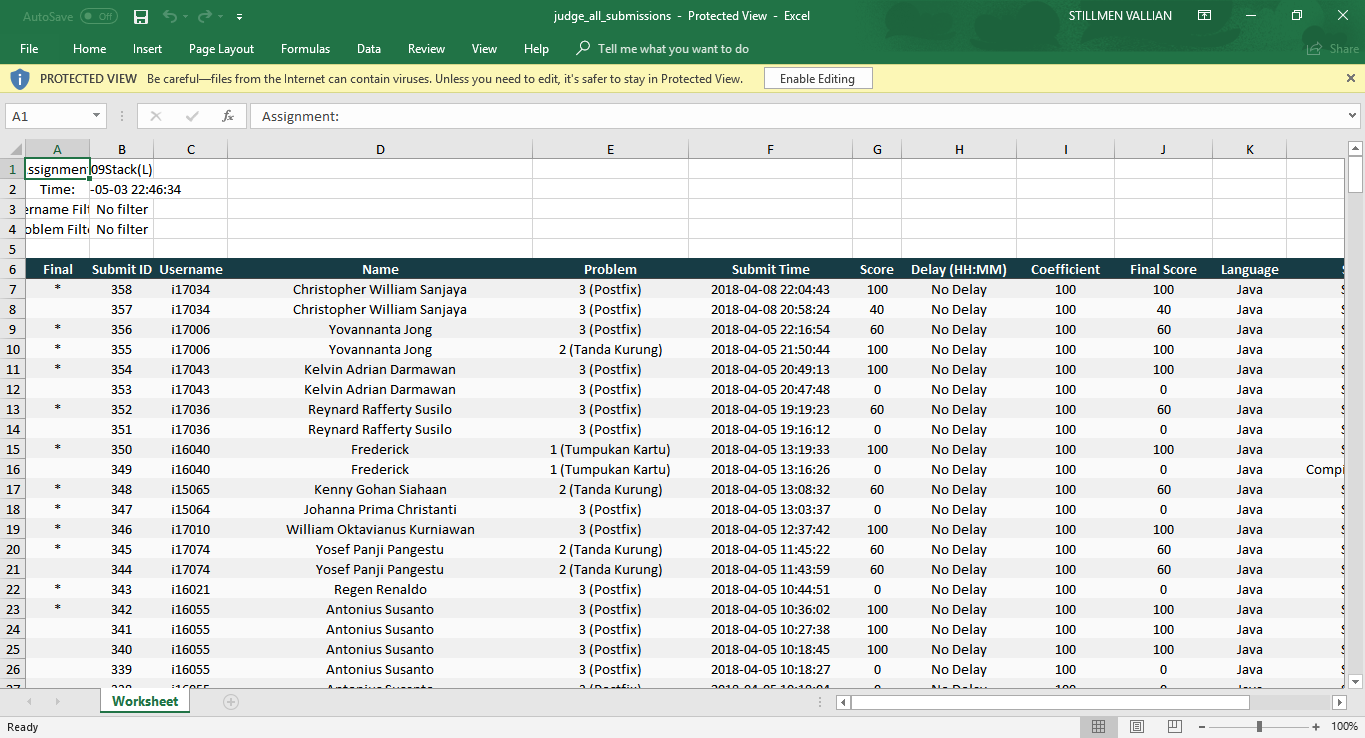
\includegraphics[width=1.0\textwidth]{/pengujian/excel/excelas}  
		\caption[Isi \textit{Excel judge\_all\_submissions.xlsx}]{Isi \textit{Excel judge\_all\_submissions.xlsx}} 
		\label{fig:excelas} 
	\end{figure}
	
	\begin{figure}[H]
		\centering  
		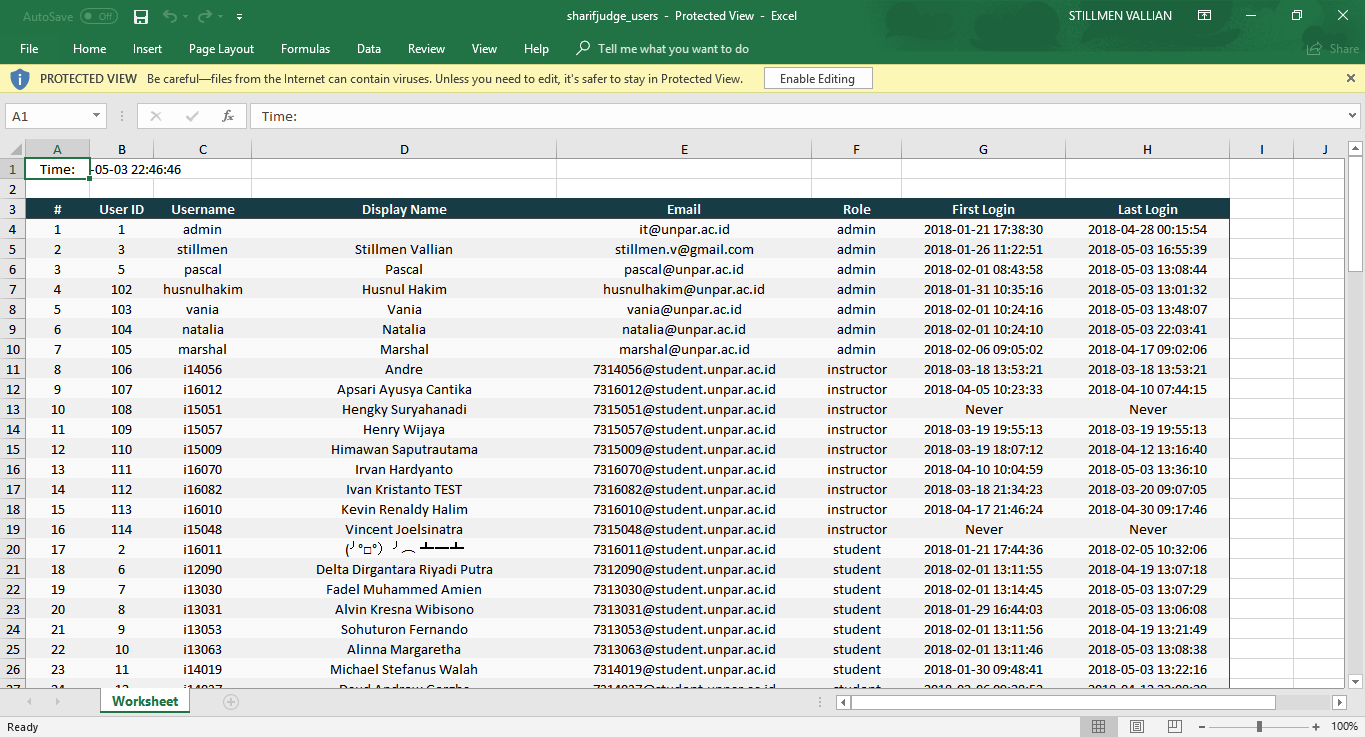
\includegraphics[width=1.0\textwidth]{/pengujian/excel/excelu}  
		\caption[Isi \textit{Excel sharifjudge\_users.xlsx}]{Isi \textit{Excel sharifjudge\_users.xlsx}} 
		\label{fig:excelu} 
	\end{figure}

\section{Analisis Dampak}
Analisis dampak pada perangkat lunak adalah proses mengidentifikasi pengaruh yang muncul dari perubahan yang telah dilakukan dan memperkirakan apa yang perlu dimodifikasi untuk mencapai perubahan~\cite{arnold:96:impact}. Perangkat lunak \textit{Sharif Judge} yang telah dikembangkan, mengalami beberapa perubahan. Beberapa perubahan tersebut yaitu:
\begin{enumerate}
	\item Basis Data \\
	Pada basis data, terdapat penambahan tabel yaitu tabel \textit{shj\_logins} dan beberapa penambahan atribut pada tabel \textit{shj\_assignments} dan \textit{shj\_settings}. Dengan adanya perubahan struktur basis data, maka proses instalasi \textit{SharIF Judge} juga berubah. Proses instalasi \textit{SharIF Judge} juga harus diperbarui agar dapat membuat basis data yang sesuai dengan hasil pengembangan.
	
	\item Tampilan \\
	Pada tampilan, terdapat penambahan halaman dan perubahan logo serta nama perangkat lunak. Beberapa halaman baru yang ditambahkan adalah halaman \textit{Hall of Fame} dan \textit{24-hour Logs}. Logo Sharif Judge diubah menggunakan logo Program Studi Teknik Informatika. Nama perangkat lunak \textit{Sharif Judge} diubah menjadi \textit{SharIF Judge}.
\end{enumerate}

\section{Masukan dari Pengguna \textit{GitHub}}
\label{sec:masukangithub}
Pada saat skripsi ini dibuat, seluruh perkembangan perangkat lunak \textit{SharIF Judge} dicommit pada repositori \textit{GitHub}. Repositori yang digunakan bersifat \textit{public}, sehingga seluruh pengguna \textit{GitHub} dapat mengakses repositori tersebut. Pengguna \textit{GitHub} dengan \textit{username} wojcik13 memberikan masukan dengan membuat \textit{issue} dengan judul "\textit{Some development proposals}" dan berkode unik \#6. Berikut isi masukan dari \textit{username} wojcik13
\begin{quote}
	``\textit{Hello,} \\
	\textit{As I see, you're developing and adding some functions to Sharif Judge, well, I'm newbie here and I don't know how to add some functions to repo. If You will have time to add them, I would be grateful.}\\
	\textit{So Ideas as following:} 
	\begin{itemize}
		\item \textit{IMO Sharif Judge should have ability to freeze scoreboard, as it is in other OJ's (DOMJudge). Usually in contest organized in Poland, it's enabled in half of contest time. }
		\item \textit{As far as I'm concerned, Sharif should have better developed permissions system. I mean, to make some groups of students, so student from group A, cannot see contest assigned to group B, and vice versa. (My idea is to add students categories, and in assignment\_edit view change participants box to Categories of students allowed to see contest) }
		\item \textit{What do You think about adding switch, which is changing judging-method? One method is already programmed by mjnaderi, and the second method is ICPC-based }
		\item \textit{Last suggestion is to precisely set publishing contests, so at setted time contest become visible, and deactivation time, so contest become invisible.}
	\end{itemize}
	\textit{I'm curious, what is Your opinion about my proposals.}\\
	\textit{Kindly regards}\\
	\textit{Wojtek Wasilewski}''
\end{quote}

%\textit{Username} wojcik13 memberikan beberapa masukan yaitu:
%\begin{itemize}
%	\item Menambahkan fungsi untuk memberhentikan scoreboard.
%	\item Menambahkan kategori student dan mengubah text area "Participant" pada halaman add atau edit assignment menjadi kategori student
%	\item Menambahkan ICPC-base judging-method
%	\item Menambahkan fungsi untuk mengatur waktu mulai dan akhir kontes.
%\end{itemize}